\documentclass[11pt,a4paper]{article}
\usepackage[T1]{fontenc}
\usepackage{fourier}
\usepackage{sectsty}
\usepackage{indentfirst}
\usepackage[pagebackref=true,breaklinks=true,colorlinks,bookmarks=false]{hyperref}
\usepackage{amsmath,amsfonts,amsthm}
\usepackage{graphicx}
\usepackage{array}
\usepackage{longtable}
\usepackage{multirow}
\usepackage{bigstrut}
\usepackage{bigdelim}
\usepackage{chngcntr}
\usepackage{framed}
\usepackage{color}
\definecolor{shadecolor}{rgb}{0.92,0.92,0.92}
\newcolumntype{M}[1]{>{\centering\arraybackslash}m{#1}}
\counterwithin{figure}{section}
\counterwithin{equation}{section}

\DeclareGraphicsExtensions{.pdf,.png}
\graphicspath{{outputs/}}

\allsectionsfont{\centering \normalfont\scshape}

\setlength\paperwidth{20.999cm}
\setlength\paperheight{29.699cm}
\setlength\voffset{-1in}
\setlength\hoffset{-1in}
\setlength\topmargin{1.499cm}
\setlength\headheight{12pt}
\setlength\headsep{0cm}
\setlength\footskip{1.131cm}
\setlength\textheight{25cm}
\setlength\oddsidemargin{2.499cm}
\setlength\textwidth{16.5cm}

\renewcommand\floatpagefraction{0.75}

\newcommand{\horrule}[1]{\rule{\linewidth}{#1}} 
\title{
		%\vspace{-1in} 	
		\usefont{OT1}{bch}{b}{n}
		\normalfont \normalsize \textsc{CS386 Digital Image Processing Autumn 2017} \\ [25pt]
		\horrule{0.5pt} \\[0.4cm]
		\huge DIP Assignment Report \\
		\horrule{2pt} \\[0.5cm]
}
\author{
		\normalfont 								\normalsize
        yelantingfeng
        \\\normalsize
		%\today
		December 31, 2017
}
\date{}

\begin{document}

\maketitle

\setcounter{section}{-1}
\section{Introduction}
Interest in digital image processing methods stems from two principal application
areas: improvement of pictorial information for human interpretation; and
processing of image data for storage, transmission, and representation for autonomous
machine perception\cite{DIP}.

This report is for the 10 assignments of digital image processing(CS386) course in SJTU, instructed
by Prof. Hongtao Lu. Files submitted together with this report are organized in this way,
 where two file folders \textbf{\emph{images}}, \textbf{\emph{outputs}} contain all used input and output images
for all 10 assignments respectively and the folder \textbf{\emph{codes}} is for all source codes of these 10
assignments. Each assignment is finished by implementing some \emph{.m} function with no use of the built-in image
processing function in Matlab. To see good results which are similar to those presented in textbook, you can directly
run the \textbf{\emph{testdemo.m}} script in every single subfolder in folder \textbf{\emph{codes}}. These scripts
will invoke those \emph{.m} functions with proper parameters and present the results in Matlab's figure windows.
If you think those images cannot be clearly browsed, you can also see the output images in \textbf{\emph{outputs}}
where the result images are saved as \emph{.png} or \emph{.pdf} files in advance.

This report will introduce the the whole 10 assignments sequentially. For each assignment, this essay
will discuss its principle, implementation and analyze its outputs. We are trying to focus on the part 
which is critical or not mentioned in textbook. To fully understand the ideas of digital image processing,
 you are still required to consult the textbook.

\section{Histogram Equalization}
\subsection{Principle}
Histogram equalization is a kind of intensity transformation which can make the PDF of an image appears more 
uniformly. With its intensity uniformly distributed, an image gets higher contrast and can be seen more clearly.
The transformation is 
\begin{equation}
	s_k=T(r_k)=\frac{L-1}{MN}\sum_{j=0}^k n_j,\quad k=0,1,2,\dots,L-1
\end{equation}
where $MN$ is the total number of pixels in the image, $n_k$ is the number of pixels with 
intensity $r_k$, and $L$ is the gray level of this image. If we apply this equation to an image, and then 
use $s_k$ to replace $r_k$, we can then get our result image.

\subsection{Implementation}
To finish this assignment, 3 functions are defined. Function \textbf{a\_histogram} is used to compute the 
histogram of an image. It has the general syntax
\begin{center}
	\textbf{[frequency, intensity] = a\_histogram(image, bitnum, plotflag)}
\end{center}
It will compute the frequency of each intensity in \textbf{image} with $2^\textbf{bitnum}$ as its gray 
level. If \textbf{plotflag} is set true, it will plot the bar chart with \textbf{frequency} and \textbf{intensity}
as its Y-axis and X-axis respectively. You can also invoke another function \textbf{plotbar} manually to 
plot the chart with command
\begin{center}
	\textbf{plotbar(intensity,frequency,bitnum)}
\end{center}
The third function is \textbf{b\_equalization} and its syntax is
\begin{center}
\textbf{[resImg, transY, transX] = b\_equalization(rawImg, bitnum, plotflag)}
\end{center}
This function will invoke \textbf{a\_histogram} to calculate the histogram of \textbf{rawImg}
and then do the transformation. \textbf{transY, transX} will be used to plot the transformation
function. By specifying a parameter \textbf{bitnum}, these functions can be applied to images 
with different gray level. %The implementation of histogram equalization is easy, so we won't talk 
%more about the implementation here.

\subsection{Result Analysis}
After running the script \textbf{testdemo.m}, you will get following results.

\begin{figure}[!htbp]
	\centering
	\begin{tabular}{cc} 
		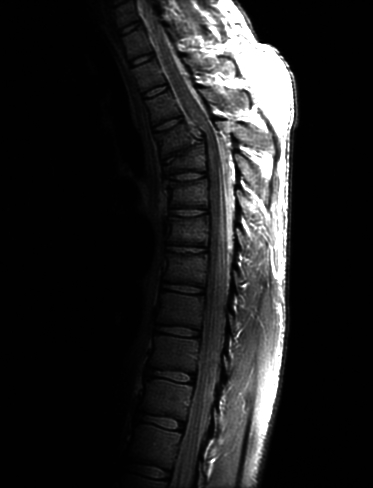
\includegraphics[width=0.3\textwidth]{pro1/fig1_origin}&
		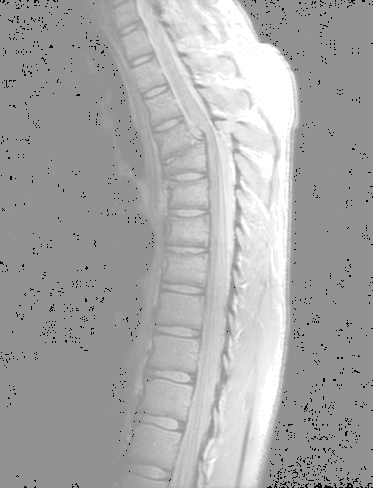
\includegraphics[width=0.3\textwidth]{pro1/fig1_enhanced} \\
		original image & enhanced image\\
		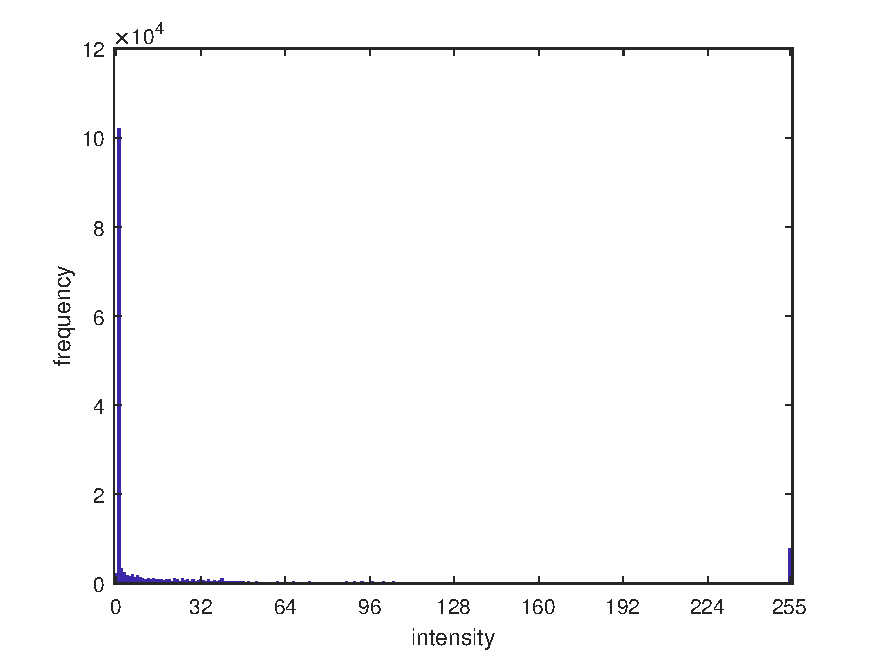
\includegraphics[width=0.4\textwidth]{pro1/fig1_originhist} &
		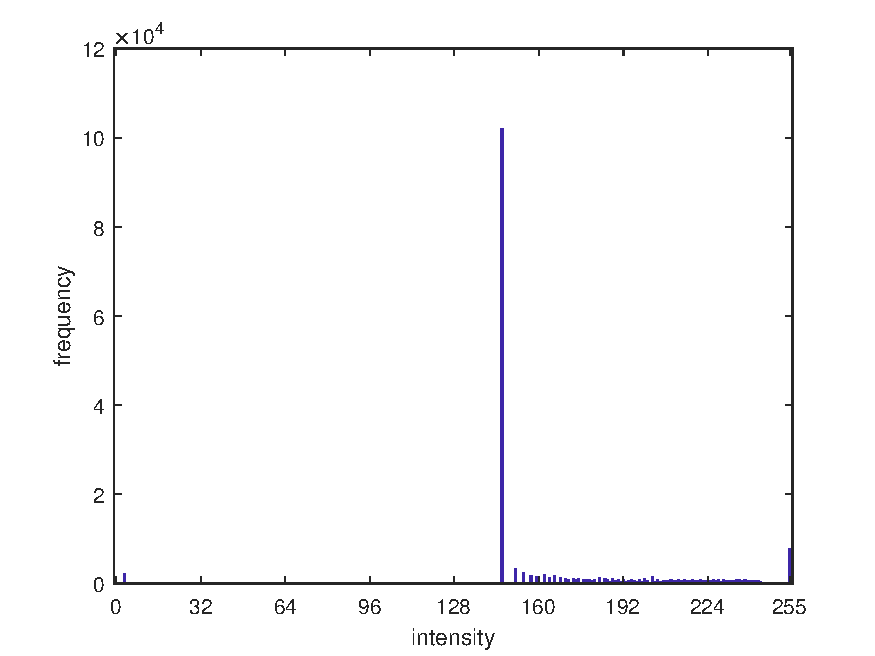
\includegraphics[width=0.4\textwidth]{pro1/fig1_enhancehist}\\
		histogram of original image & histogram of enhanced image
	\end{tabular}
	\caption{Result of \textbf{fig1.jpg}}
	\label{pro1_fig1}
\end{figure}

As we can see in
Figure \ref{pro1_fig1}, for the first test image \textbf{fig1.jpg}, this method doesn't work well
enough. Though more details can be seen in enhanced image, it looks overexposed since there is a 
large white area in it. This is because we are dealing with discrete values. You can also find this 
problem correspondingly by observe the histogram plot of enhance image. Figure \ref{pro1_fig2} shows
the transformation function.

\begin{figure}[!htbp]
	\centering
	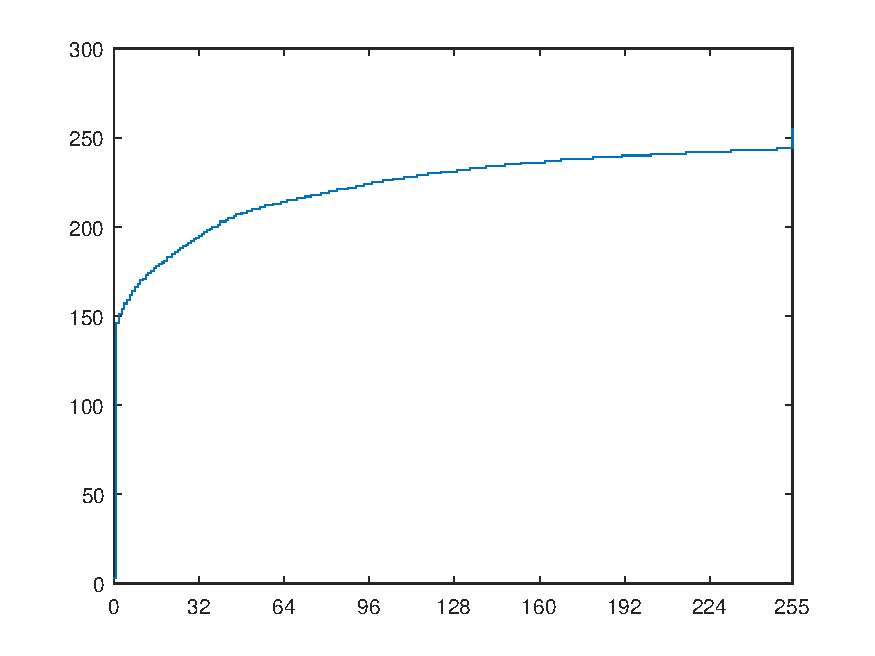
\includegraphics[width=0.8\textwidth]{pro1/fig1_trans}
	\caption{Transformation function of \textbf{fig1.jpg}}
	\label{pro1_fig2}
\end{figure}

\begin{figure}[!htbp]
	\centering
	\begin{tabular}{cc} 
		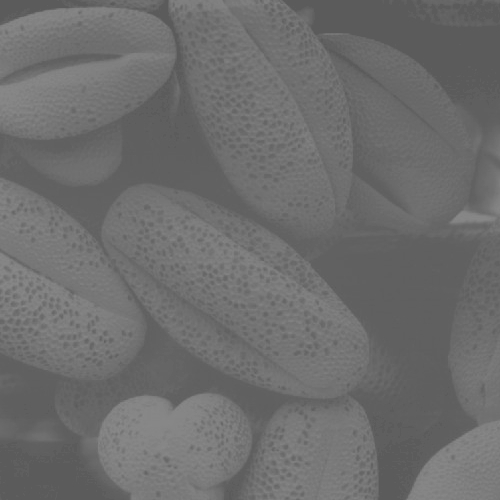
\includegraphics[width=0.3\textwidth]{pro1/fig2_origin}&
		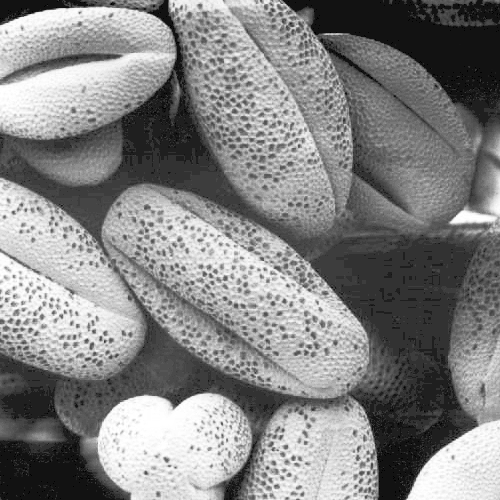
\includegraphics[width=0.3\textwidth]{pro1/fig2_enhanced} \\
		original image & enhanced image\\
		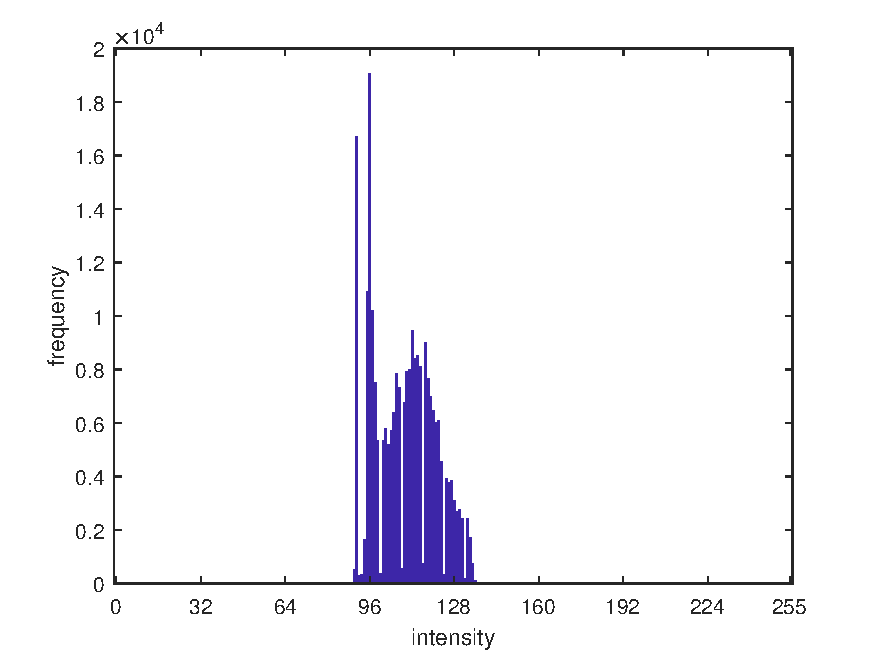
\includegraphics[width=0.4\textwidth]{pro1/fig2_originhist} &
		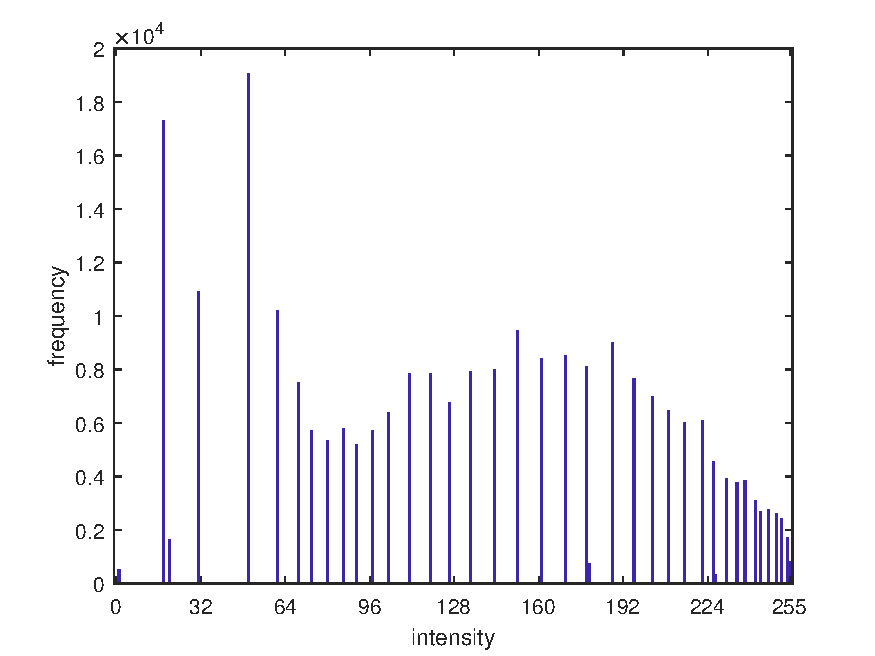
\includegraphics[width=0.4\textwidth]{pro1/fig2_enhancehist}\\
		histogram of original image & histogram of enhanced image
	\end{tabular}
	\caption{Result of \textbf{fig2.jpg}}
	\label{pro1_fig3}
\end{figure}

The second test image \textbf{fig2.jpg} performs better, as you can see in Figure \ref{pro1_fig3}. 
After histogram equalization, the histogram of the image becomes much more uniform. The enhanced 
image looks accordingly better than that of \textbf{fig1.jpg}. The result of this test image can 
be found as \textbf{FIGURE 3.20} in the textbook. Our result is nearly the same with that. The transformation
 function is displayed in Figure \ref{pro1_fig4}.

\begin{figure}[!htbp]
	\centering
	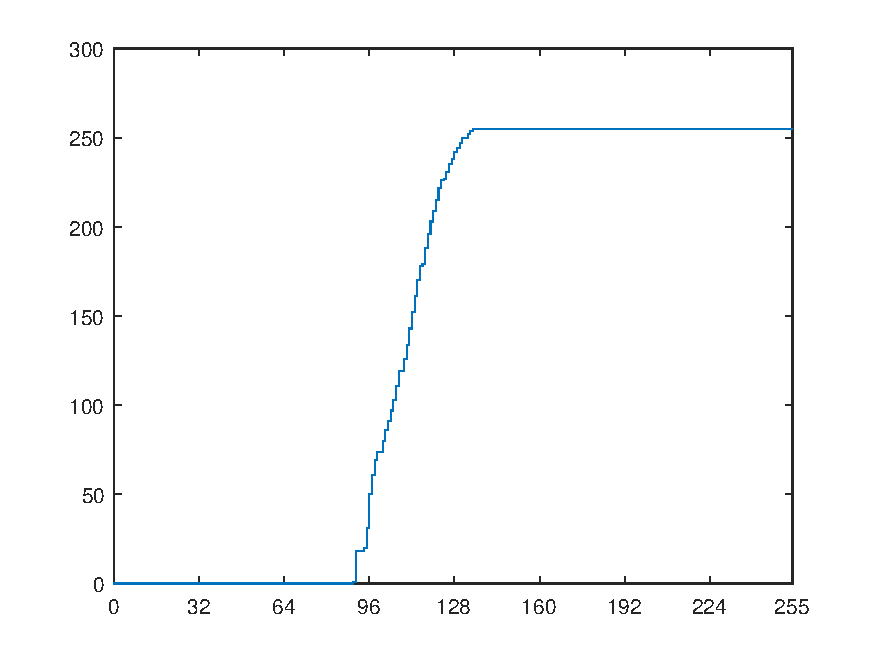
\includegraphics[width=0.8\textwidth]{pro1/fig2_trans}
	\caption{Transformation function of \textbf{fig2.jpg}}
	\label{pro1_fig4}
\end{figure}

\section{Combining spatial enhancement methods}
\subsection{Principle}
In this assignment, we are required to enhance an image by using diffrent kinds of enhancement methods
sequentially. These methods include Laplacian, Sobel gradient, averaging filter, power-law
 transformation and simple array operation(addtion and multiplication). 

Laplacian and gradient are two types of sharpening filters which are based on first-order and second-order
derivatives respectively. Laplacian of two variables is
\begin{equation}
	\nabla^2 f(x,y)=f(x+1,y)+f(x-1,y)+f(x,y+1)+f(x,y-1)-4f(x,y)
\end{equation}
The gradient of $f(x,y)$ is a vector which defined as 
\begin{equation}
\nabla f\equiv grad(f)\equiv\left[\begin{array}{c}g_x \\ g_y\end{array}\right]
	\equiv\left[\begin{array}{c}
		\frac{\partial f}{\partial x} \\ 
		\frac{\partial f}{\partial y}
	\end{array}	\right]
\end{equation}
Sobel gradient calculate $g_x$ and $g_y$ in this way where
\begin{equation}
	g_x=\frac{\partial f}{\partial x}=(z_7+2z_8+z_9)-(z_1+2z_2+z_3)
\end{equation}
and
\begin{equation}
	g_y=\frac{\partial f}{\partial y}=(z_3+2z_6+z_9)-(z_1+2z_4+z_7)
\end{equation}
$z_k(k=1,2,\dots,4,6,\dots,9)$ here denote eight neighbors of $f(x,y)=z_5$. Indices 
are given from left to right and top to bottomn. Its magnitude can be calculated following
\begin{equation}
	M(x,y)=|g_x|+|g_y|
\end{equation}

Averaging filtering is a linear filter where value of each pixel will be the average of its neighbors.

Power-law transformation is a kind of intensity transform with the form
\begin{equation}
	s=cr^{\gamma}
\end{equation}
where $r$ is the raw intensity value, and $s$ is the transformation of $r$.

\subsection{Implementation}
For power-law transformation and simple array operation, the implementation is 
quite easy. The critical part of this assignment is to implement a linear filter
which can be specified with different masks. Once done, the Laplacian, Sobel gradient
and averaging filter can be easily computed.

Linear filter implemented here is a function called \textbf{dipLinearFilter}.
You can invoke it with the syntax
\begin{center}
	\textbf{[resImg] = dipLinearFilter(rawImg, mask)}
\end{center}
where \textbf{rawImg} is the target image data, and \textbf{mask} is a filter mask
stored in a 2-D matrix. Output \textbf{resImg} is the result of filtering contains 
values in double type. This function is implemented with zero padded and don not use 
the built-in function \textbf{conv2}. Thus, the speed is a little slower but still 
tolerable. For masks used for different methods, you can see them in Figure \ref{pro2_masks}.

\begin{figure}[!htbp]
	\centering
	\begin{tabular}{c|c|cc}
		$\frac{1}{25}$
\setlength\tabcolsep{0pt}
\begin{tabular}{|@{\rule[-0.4cm]{0pt}{1cm}}*{5}{M{1cm} |}}
	\hline
1 & 1 & 1 & 1 & 1 \\
	\hline
1 & 1 & 1 & 1 & 1 \\
	\hline
1 & 1 & 1 & 1 & 1\\
	\hline
1 & 1 & 1 & 1 & 1\\
	\hline
1 & 1 & 1 & 1 & 1\\
	\hline
	\end{tabular}&
\setlength\tabcolsep{0pt}
\begin{tabular}{|@{\rule[-0.4cm]{0pt}{1cm}}*{3}{M{1cm} |}}
	\hline
0 & -1 & 0 \\
	\hline
-1 & 4 & -1 \\
	\hline
0 & -1 & 0 \\
	\hline
	\end{tabular} & 
\setlength\tabcolsep{0pt}
\begin{tabular}{|@{\rule[-0.4cm]{0pt}{1cm}}*{3}{M{1cm} |}}
	\hline
-1 & -2 & -1 \\
	\hline
0 & 0 & 0 \\
	\hline
1 & 2 & 1 \\
	\hline
	\end{tabular} &
\setlength\tabcolsep{0pt}
\begin{tabular}{|@{\rule[-0.4cm]{0pt}{1cm}}*{3}{M{1cm} |}}
	\hline
-1 & 0 & 1 \\
	\hline
-2 & 0 & 2 \\
	\hline
-1 & 0 & 1 \\
	\hline
	\end{tabular}\\
	$5\times 5$ averaging filter &
	Laplacian & Sobel gradient($g_x$) & Sobel gradient($g_y$)
\end{tabular}
	\caption{Masks we used}
	\label{pro2_masks}
\end{figure}

\subsection{Resutl Analysis}
After running the script \textbf{testdemo.m}, you will get following results.

\begin{figure}[!htbp]
	\centering
	\begin{tabular}{cccc} 
		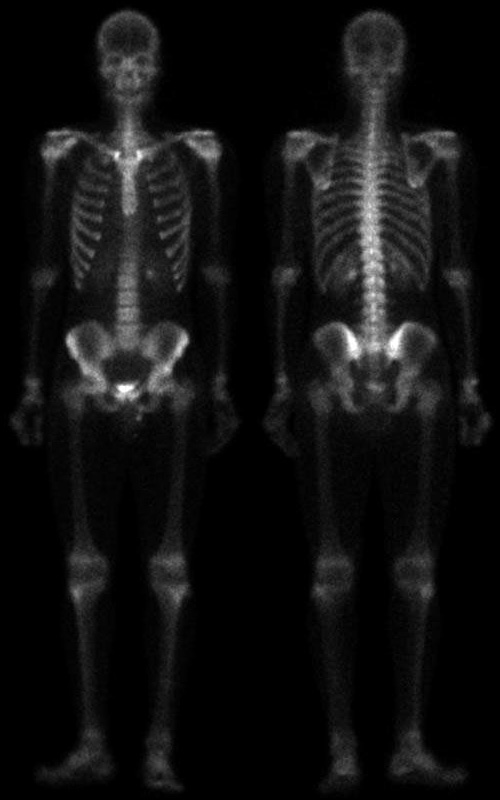
\includegraphics[width=0.2\textwidth]{pro2/a}&
		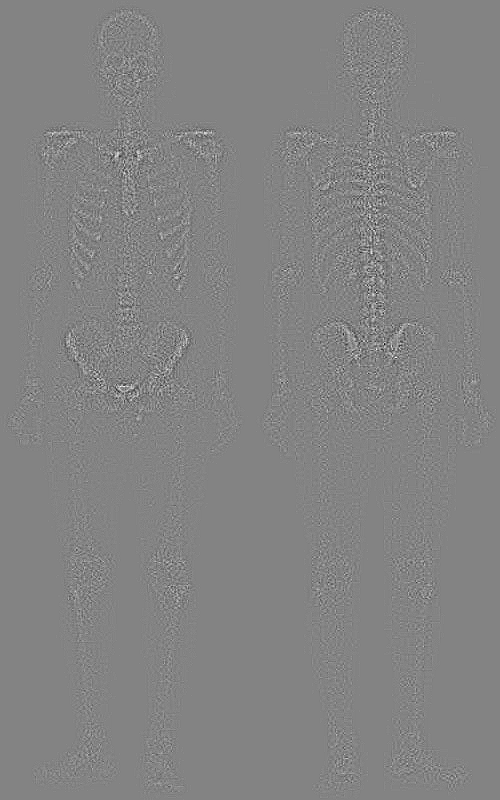
\includegraphics[width=0.2\textwidth]{pro2/b}&
		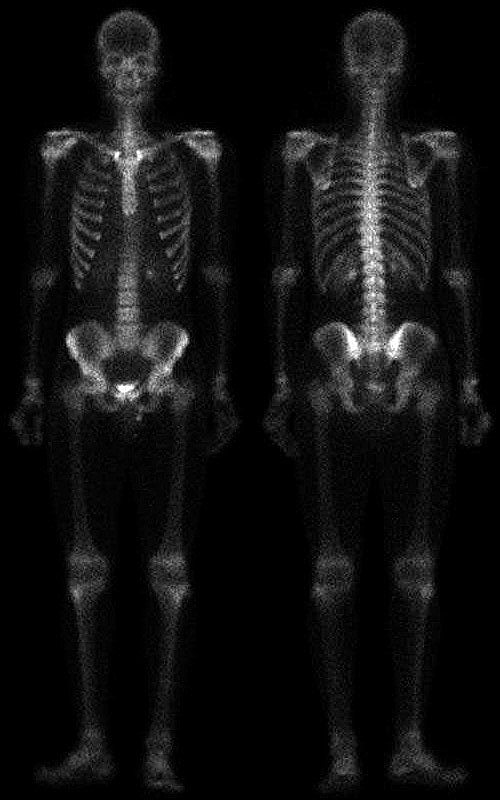
\includegraphics[width=0.2\textwidth]{pro2/c}&
		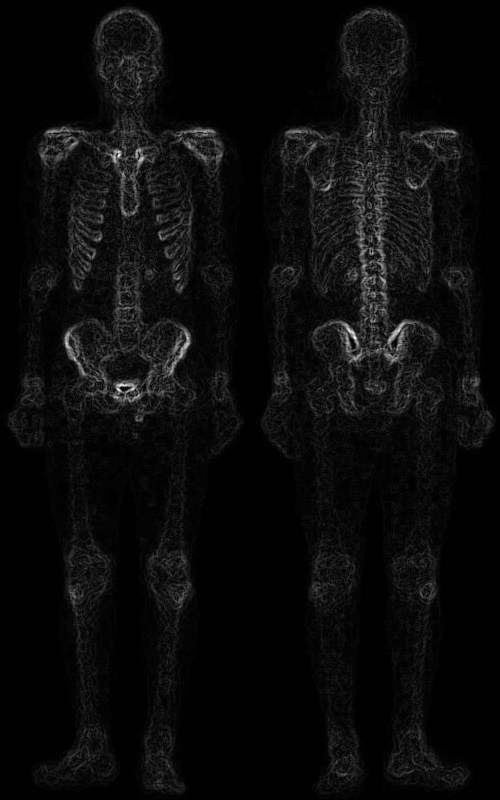
\includegraphics[width=0.2\textwidth]{pro2/d} \\
		(a) original image & (b) Laplacian of (a) & (c) Sum of (a) and (b)
		& (d) Sobel of (a)\\
		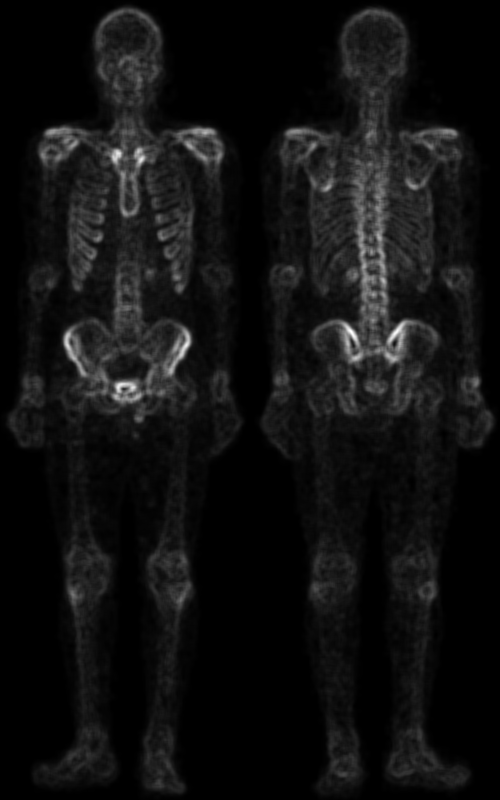
\includegraphics[width=0.2\textwidth]{pro2/e}&
		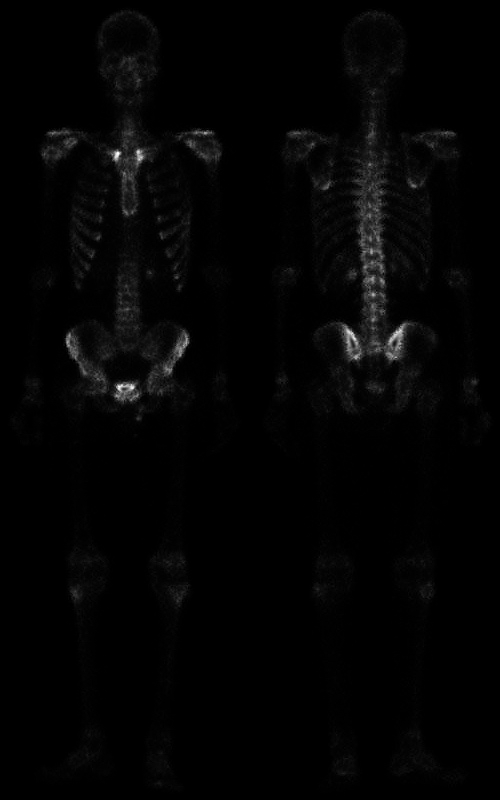
\includegraphics[width=0.2\textwidth]{pro2/f}&
		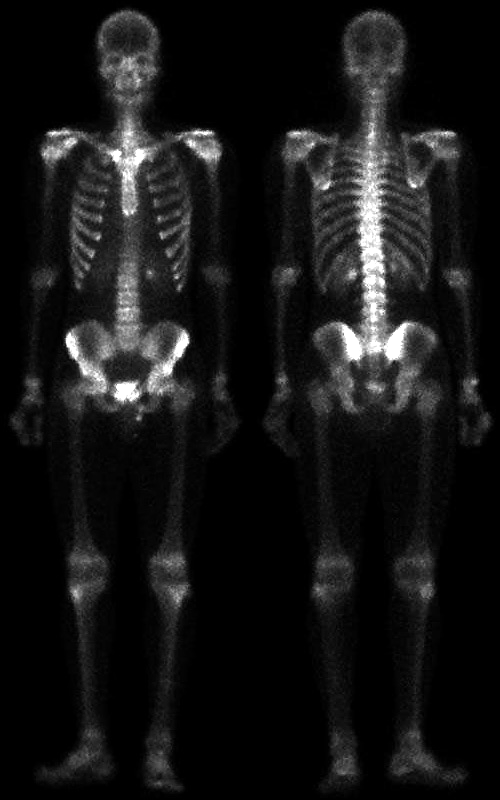
\includegraphics[width=0.2\textwidth]{pro2/g}&
		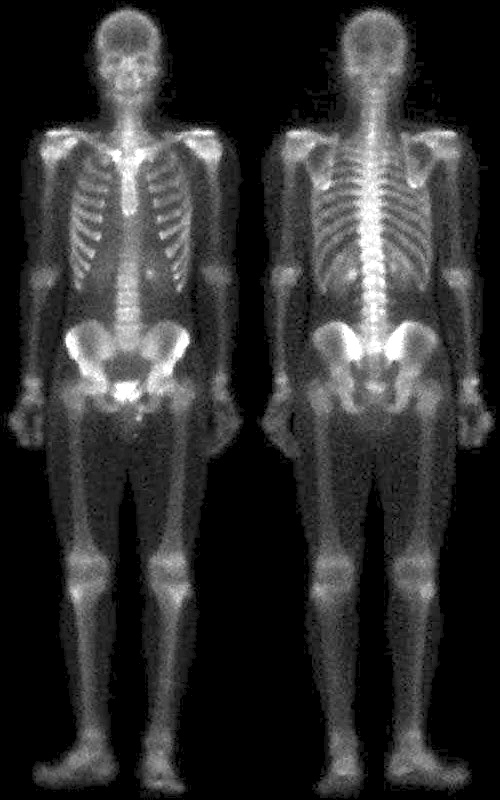
\includegraphics[width=0.2\textwidth]{pro2/h} \\
		(e) averaging of (d) & (f) Product of (c),(e) & (g) Sum of (a) and (f)
		& (h) power-law of (g)
	\end{tabular}
	\caption{Enhancement of \textbf{skeleton\_orig.tif}}
	\label{pro2_fig1}
\end{figure}

In Figure \ref{pro2_fig1}, we can see that in the final result (h), we see that significant new
detail is visible. The areas around the wrists, hands, ankles, and
feet are good examples of this. The skeletal bone structure also is much more
pronounced, including the arm and leg bones. Note also the faint definition of
the outline of the body, and of body tissue. Bringing out detail of this nature by
expanding the dynamic range of the intensity levels also enhanced noise, but it still 
represents a significant visual improvement over the original image \textbf{skeleton\_orig.tif}.
The result of this test image can be found as \textbf{FIGURE 3.43} in the textbook.

\section{Filtering in frequency domain}
\subsection{Principle}

Filtering techniques in the frequency domain are based on modifying the
Fourier transform to achieve a specific objective and then computing the inverse
DFT to get us back to the image domain.

2-D discrete Fourier transform(DFT) is 
\begin{equation}
	F(u,v)=\sum_{x=0}^{M-1}\sum_{y=0}^{N-1}f(x,y)e^{-j2\pi(ux/M+vy/N)}
\end{equation}
and the inverse discrete Fourier transform(IDFT) is
\begin{equation}
	F(u,v)=\frac{1}{MN}\sum_{u=0}^{M-1}\sum_{v=0}^{N-1}F(u,v)e^{j2\pi(ux/M+vy/N)}
\end{equation}

Steps for Filtering in the Frequency Domain are as follows:
\begin{enumerate}
	\item Given an input image of $f(x,y)$ of size $M\times N$, obtain the padding
	parameters $P$ and $Q$ where $P\geq 2M-1$ and $Q\geq 2N-1$. This is to avoid wraparound error.
	\item Form a padded image, $f_p(x,y)$, of size $P\times Q$ by appending the 
	necessary number of zeros to $f(x,y)$.
	\item Multiply $f_p(x,y)$ by $(-1)^{x+y}$ to center its transform.
	\item Compute the DFT, $F(u,v)$, of the image of step 3.
	\item Generate a real, symmetric filter function, $H(u,v)$, of size $P\times Q$
	with center at coordinates $(P/2,Q/2)$. Form the product $G(u,v)=H(u,v)F(u,v)$
	using array multiplication; that is, $G(i,k)=H(i,k)F(i,k)$.
	\item Obtain the processed image:
	\begin{equation}
		g_p(x,y)=\left\{real\left[\mathcal{F}^{-1}\left[G(u,v)\right]\right]\right\}(-1)^{x+y}
	\end{equation}
	where the real part is selected in order to ignore parasitic complex components
	resulting from computational inaccuracies, and the subscript p indicates
	that we are dealing with padded arrays.
	\item Obtain the final processed result, $g(x,y)$, by extracting the $M\times N$ region
	from the top,left quadrant of $g_p(x,y)$.
\end{enumerate}

We are required to implement 6 kinds of filters in this assignment, 3 of them are lowpass
and the other 3 are highpass. All these filters are dependent by the function $D(u,v)$,
where 
\begin{equation}
	D(u,v)=\left[(u-P/2)^2+(v-Q/2)^2\right]^{1/2}
\end{equation}

Each type of filters are defined as follows:
\begin{enumerate}
	\item ideal lowpass filter(ILPF)
	\begin{equation}
	H(u,v)=\left\{\begin{array}{ll}
		1,&D(u,v)\leq D_0\\
		0,&D(u,v)>D_0
	\end{array}\right.
\end{equation}
	\item ideal highpass filter(IHPF)
	\begin{equation}
		H(u,v)=\left\{\begin{array}{ll}
			0,&D(u,v)\leq D_0\\
			1,&D(u,v)>D_0
		\end{array}\right.
	\end{equation}
	\item Butterworth lowpass filter(BLPF)
	\begin{equation}
		H(u,v)=\frac{1}{1+\left[D(u,v)/D_0\right]^{2n}}
	\end{equation}
	\item Butterworth highpass filter(BHPF)
	\begin{equation}
		H(u,v)=1-\frac{1}{1+\left[D(u,v)/D_0\right]^{2n}}=\frac{1}{1+\left[D_0/D(u,v)\right]^{2n}}
	\end{equation}
	\item Gaussian lowpass filter(GLPF)
	\begin{equation}
		H(u,v)=e^{-D^2(u,v)/2D_0^2}
	\end{equation}
	\item Gaussian highpass filter(GHPF)
	\begin{equation}
		H(u,v)=1-e^{-D^2(u,v)/2D_0^2}
	\end{equation}
\end{enumerate}

\subsection{Implementation}
To finish the task in this assignment, we first need to implement the DFT and IDFT function.
Rather than use the built-in function \textbf{fft2} and \textbf{ifft2}, I implement 
my own function \textbf{dip2DDFT.m} and \textbf{dip2DIDFT.m}. These two functions are implemented
as naive DFT and IDFT, instead of FFT and IFFT, which are not introduced in our textbook. However,
the implementation are well coded to use matrix multiplication, which can accelerate these functions
to a large extent. Though they are still much slower than \textbf{fft2} and \textbf{ifft2}, but I believe the 
thinking behind these two functions still counts, which may also be applied to implement FFT and
IFFT.

The idea is to use the separability of the 2-D DFT, and then it can be write as 
\begin{equation}
	F(u,v)=\sum_{x=0}^{M-1}e^{-j2\pi ux/M}\sum_{y=0}^{N-1}f(x,y)e^{-j2\pi vy/N}
\end{equation}
By observing this equation and thinking a little more, you will found that the result
can be calculated by constructing 2 matrices \textbf{A} and \textbf{B}, and 
then you just need to multiply them, \emph{s.t.}
\begin{equation}
	\mathbf{F}=\mathbf{AfB}
\end{equation}
The structure of matrices are displayed in Figure \ref{pro3_mat}, where 
\begin{equation}
	g(u,x)=e^{-j2\pi ux/M}
\end{equation}
and
\begin{equation}
	h(y,v)=e^{-j2\pi vy/N}
\end{equation}

\begin{figure}[!htbp]
	\centering
	\begin{tabular}{ccc}
		$x$&$y$&$v$\\
		$u$
		\setlength\tabcolsep{0pt}
		\scriptsize
\begin{tabular}{|@{\rule[-0.4cm]{0pt}{1cm}}*{5}{M{1cm} |}}
	\hline
$g(0,0)$ & $g(0,1)$ & ... & $g(0,M-2)$ & $g(0,M-1)$ \\
	\hline
$g(1,0)$ & ... & ... & ... & $g(1,M-1)$ \\
	\hline
... & ... & $g(u,x)$ & ... & ...\\
	\hline
$g(M-2,0)$ & ... & ... & ... & $g(M-2,M-1)$\\
	\hline
$g(M-1,0)$ & $g(M-1,1)$ & ... & $g(M-1,M-2)$ & $g(M-1,M-1)$\\
	\hline
	\end{tabular}&
	$x$
	\setlength\tabcolsep{0pt}
	\scriptsize
\begin{tabular}{|@{\rule[-0.4cm]{0pt}{1cm}}*{5}{M{1cm} |}}
	\hline
$f(0,0)$ & $f(0,1)$ & ... & $f(0,N-2)$ & $f(0,N-1)$ \\
	\hline
$f(1,0)$ & ... & ... & ... & $f(1,N-1)$ \\
	\hline
... & ... & $f(x,y)$ & ... & ...\\
	\hline
$f(M-2,0)$ & ... & ... & ... & $f(M-2,N-1)$\\
	\hline
$f(M-1,0)$ & $f(M-1,1)$ & ... & $f(M-1,N-2)$ & $f(M-1,N-1)$\\
	\hline
	\end{tabular}&
	$y$
	\setlength\tabcolsep{0pt}
	\scriptsize
\begin{tabular}{|@{\rule[-0.4cm]{0pt}{1cm}}*{5}{M{1cm} |}}
	\hline
$h(0,0)$ & $h(0,1)$ & ... & $h(0,N-2)$ & $h(0,N-1)$ \\
	\hline
$h(1,0)$ & ... & ... & ... & $h(1,N-1)$ \\
	\hline
... & ... & $h(y,v)$ & ... & ...\\
	\hline
$h(N-2,0)$ & ... & ... & ... & $h(N-2,N-1)$\\
	\hline
$h(N-1,0)$ & $h(N-1,1)$ & ... & $h(N-1,N-2)$ & $h(N-1,N-1)$\\
	\hline
	\end{tabular}\\
	$\mathbf{A}(M\times M)$&
	$\mathbf{f}(M\times N)$&
	$\mathbf{B}(N\times N)$
	\end{tabular}
	\caption{Structure of matrices}
	\label{pro3_mat}
\end{figure}

Once we implement DFT in this way, we can caculate IDFT use DFT as follows:
\begin{equation}
	f(x,y)=\frac{1}{MN}\left(\mathcal{F}\left(F^*(u,v)\right)\right)^*
\end{equation}
$F^*$ means the complex conjugate of $F$.

After DFT and IDFT is implemented, we only need to apply different filter function
$H$ to the frequency domain of the image, and every step is done following the steps
mentioned above. Finally we can get the expected result.

\subsection{Result Analysis}
After running the script \textbf{testdemo.m}, you will get six groups of results.
Each group are result of one kind of filter under different parameters. Only part of 
results are presented here, you can browse all results by running \textbf{testdemo.m} or
look into the file folder \textbf{./outputs/pro3/}.

As you can see in Figure \ref{pro3_fig1}, ILPF blurs the original image to different extents
when specifying different $D_0$. The blurring and ringing properties of ILPFs can be explained using the
convolution theorem. The result displayed in Figure \ref{pro3_fig2} is in frequency domiain,
where some circles with different radius and same center point can be easily found. Simlularly, 
Figure \ref{pro3_fig3} and \ref{pro3_fig4} presented the result of GLPF. You can find some differences
between these two groups of results.

Results of BHPF with $n=2$ are presented in Figure \ref{pro3_fig5} and \ref{pro3_fig6}. These result images in 
spatial domain are sharpened to different extents, which is exactly what is highpass filter doing.

You can compare these results with the images presented in section 4.8-4.9 of the textbook, the similarity between
them will announce the correctness of our results.

\begin{figure}[!htbp]
	\centering
	\begin{tabular}{ccc} 
		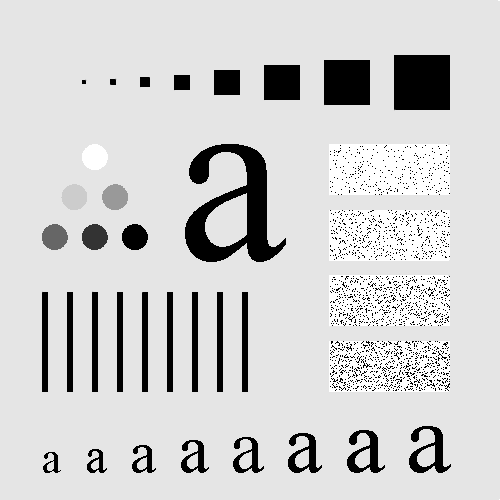
\includegraphics[width=0.3\textwidth]{pro3/org}&
		
\includegraphics[width=0.3\textwidth]{pro3/ILPF/ILPF_10}&
		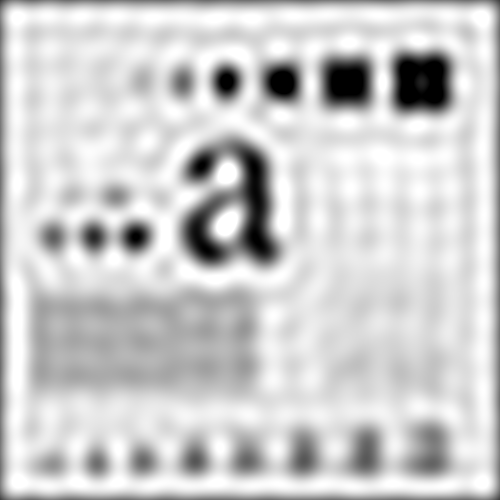
\includegraphics[width=0.3\textwidth]{pro3/ILPF/ILPF_30} \\
		original image &  $D_0=10$ &  $D_0=30$\\
		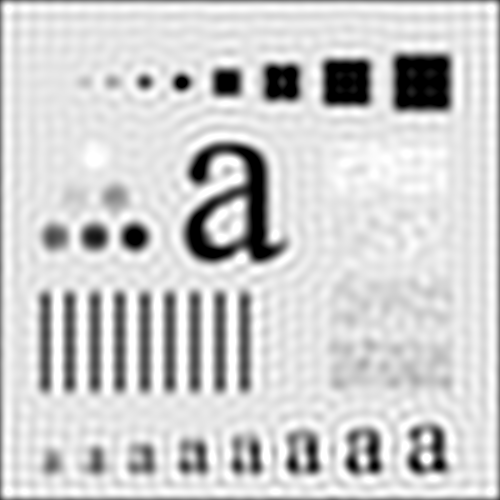
\includegraphics[width=0.3\textwidth]{pro3/ILPF/ILPF_60}&
		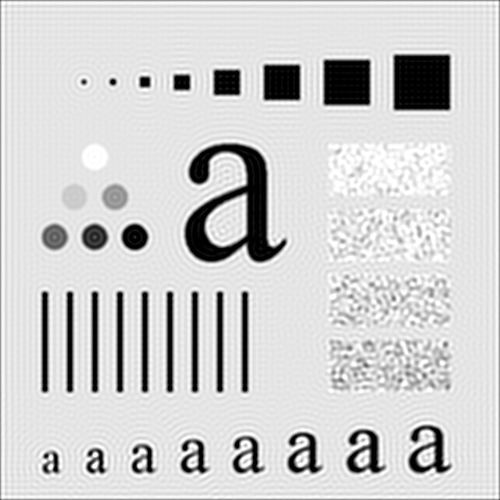
\includegraphics[width=0.3\textwidth]{pro3/ILPF/ILPF_160}&
		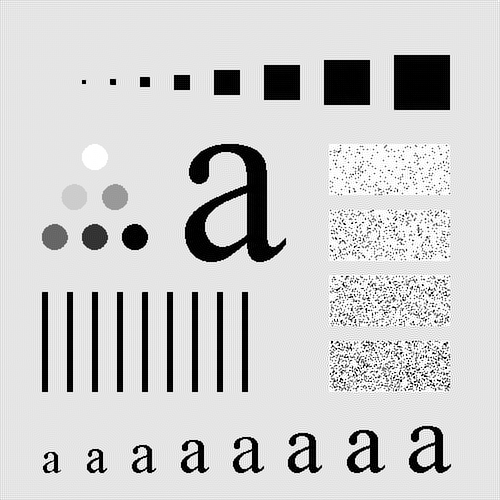
\includegraphics[width=0.3\textwidth]{pro3/ILPF/ILPF_460} \\
		 $D_0=60$ &  $D_0=160$ &  $D_0=460$
	\end{tabular}
	\caption{ILPF result of \textbf{characters\_test\_pattern.tif} in spatial domain}
	\label{pro3_fig1}
\end{figure}

\begin{figure}[!htbp]
	\centering
	\begin{tabular}{ccc} 
		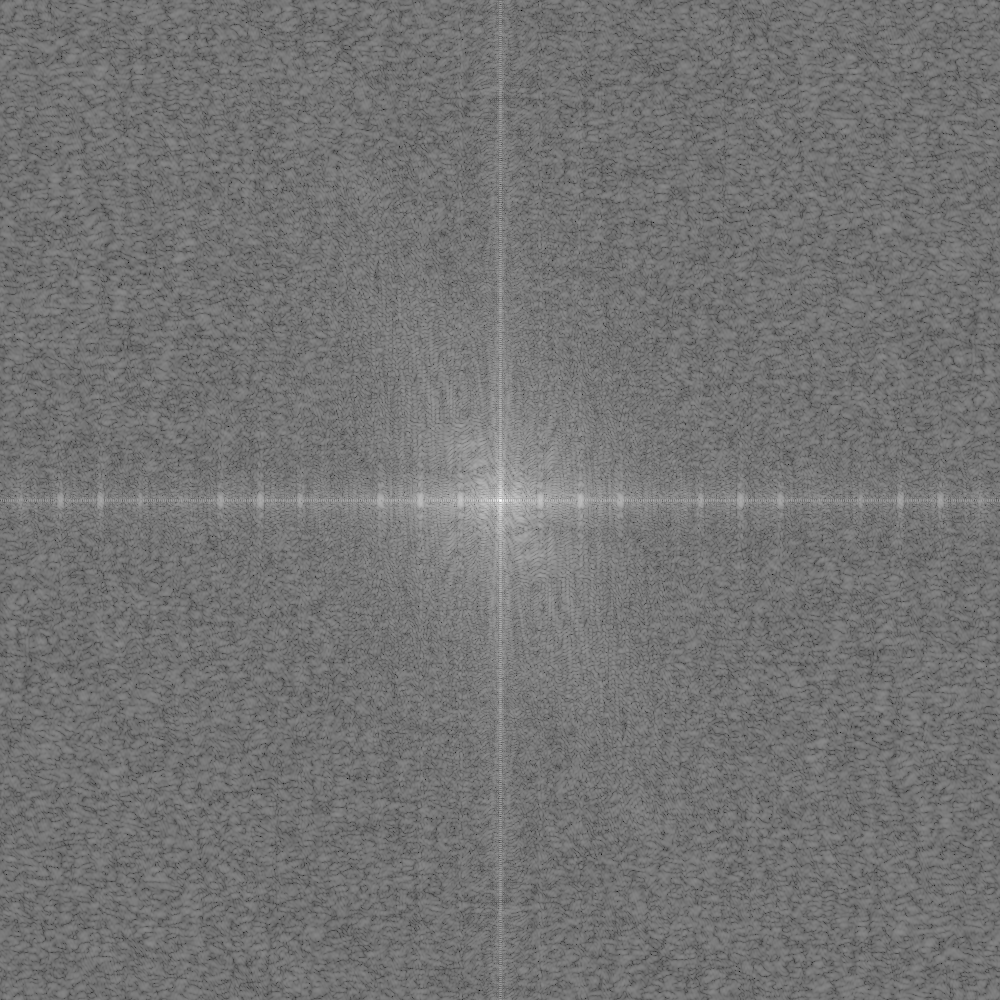
\includegraphics[width=0.3\textwidth]{pro3/org_spectrum}&
		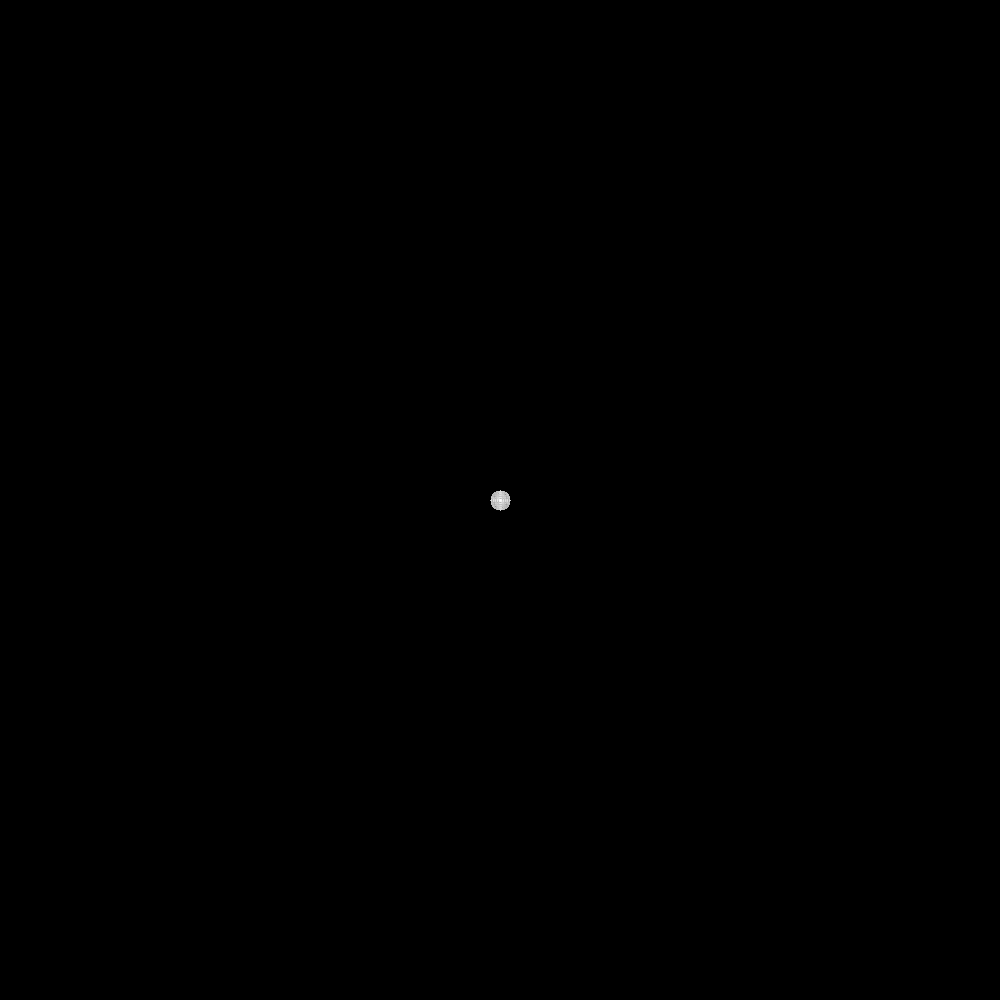
\includegraphics[width=0.3\textwidth]{pro3/ILPF/ILPF_10_spectrum}&
		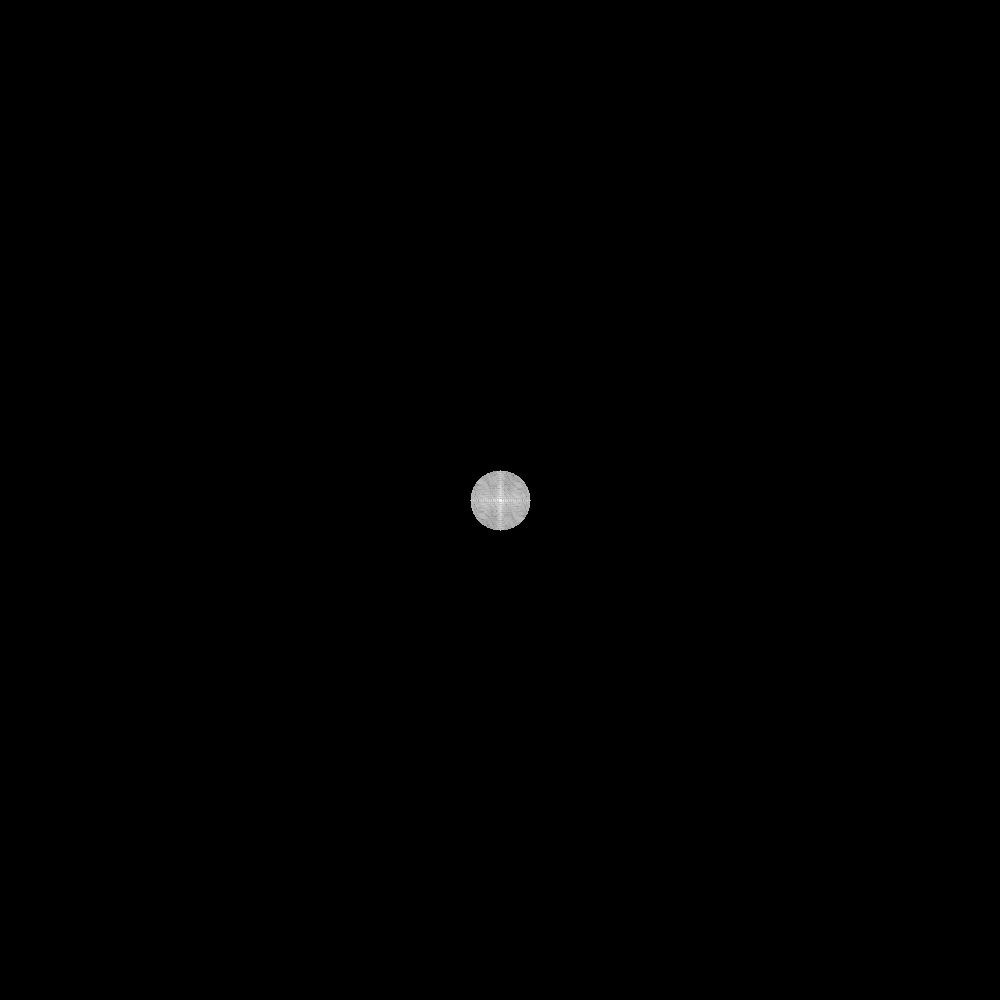
\includegraphics[width=0.3\textwidth]{pro3/ILPF/ILPF_30_spectrum} \\
		original image &  $D_0=10$ &  $D_0=30$\\
		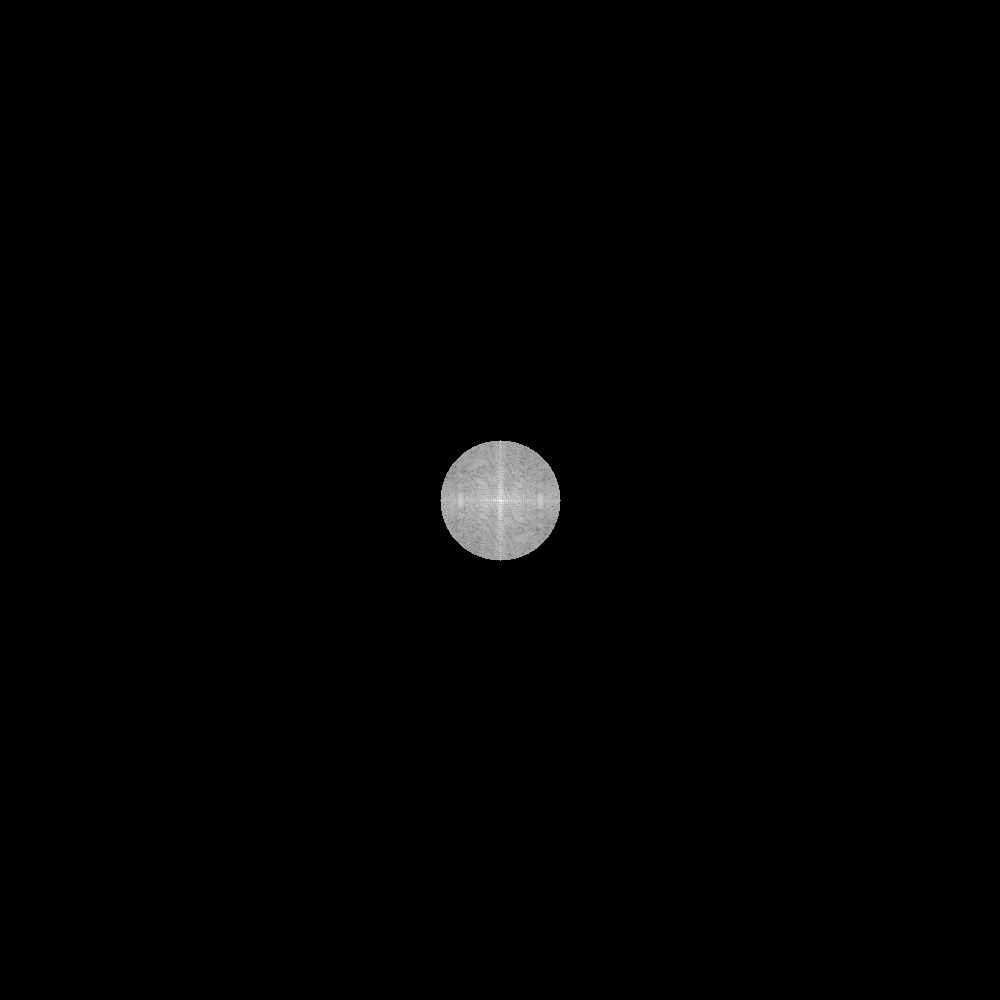
\includegraphics[width=0.3\textwidth]{pro3/ILPF/ILPF_60_spectrum}&
		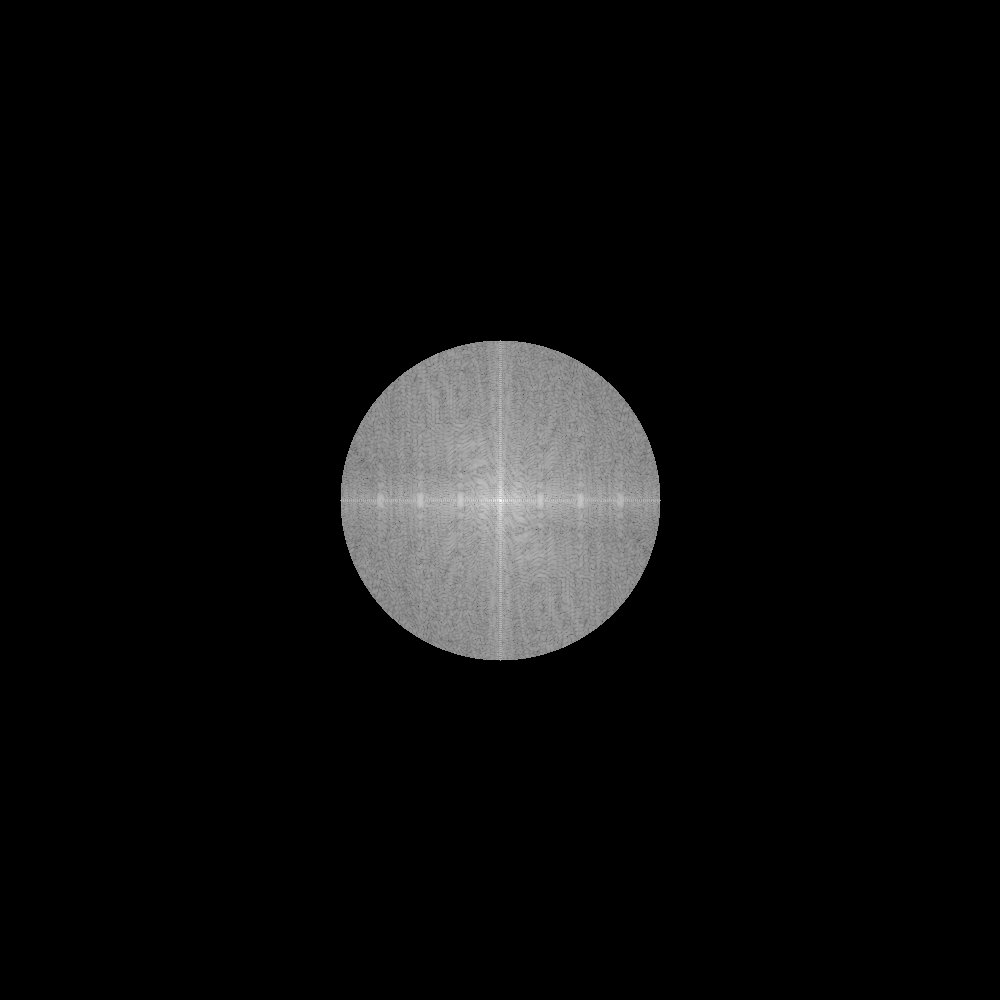
\includegraphics[width=0.3\textwidth]{pro3/ILPF/ILPF_160_spectrum}&
		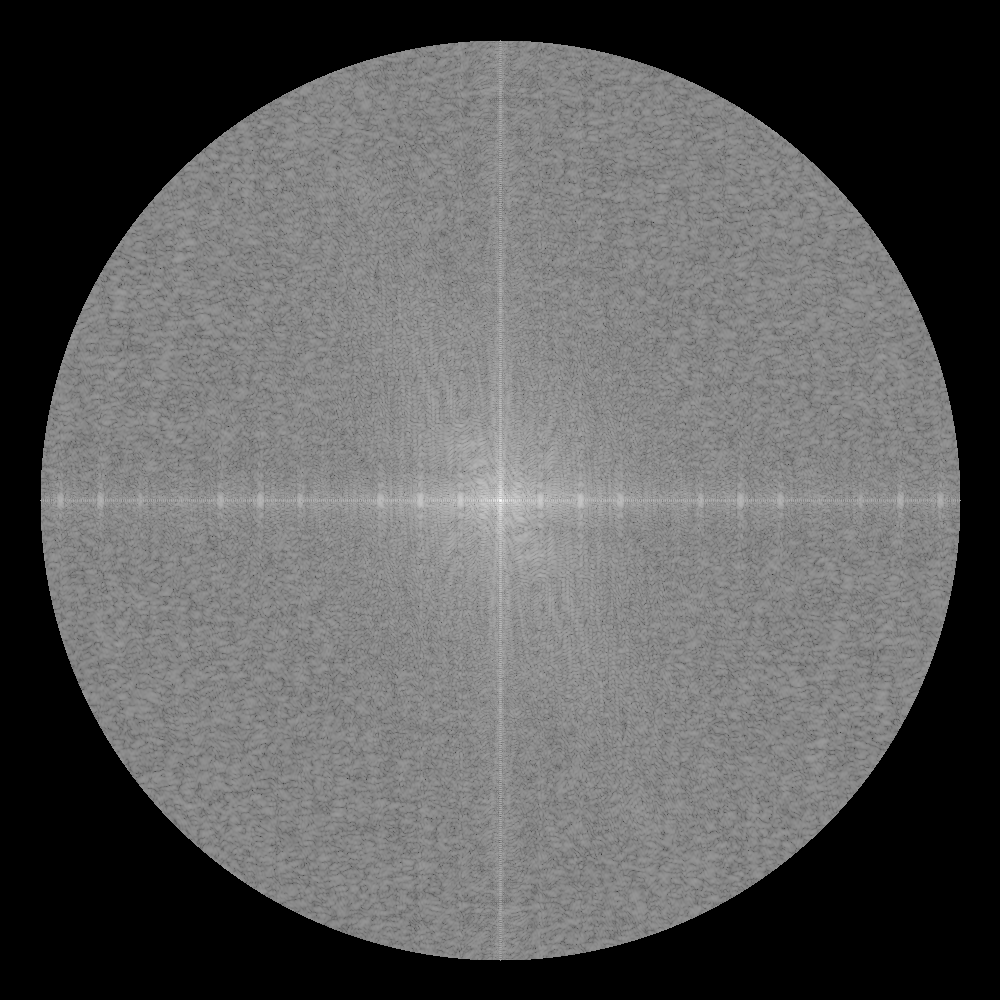
\includegraphics[width=0.3\textwidth]{pro3/ILPF/ILPF_460_spectrum} \\
		 $D_0=60$ &  $D_0=160$ &  $D_0=460$
	\end{tabular}
	\caption{ILPF result of \textbf{characters\_test\_pattern.tif} in frequency domain}
	\label{pro3_fig2}
\end{figure}

\begin{figure}[!htbp]
	\centering
	\begin{tabular}{ccc} 
		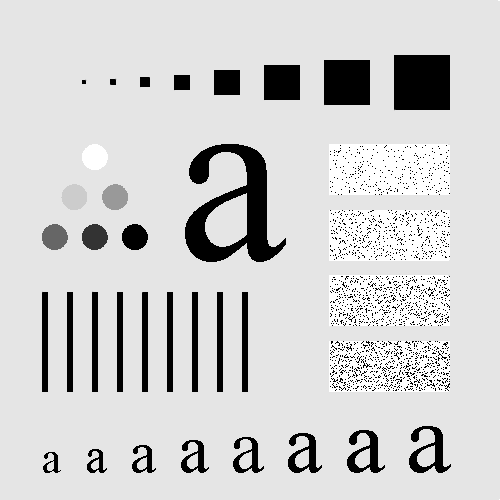
\includegraphics[width=0.3\textwidth]{pro3/org}&
		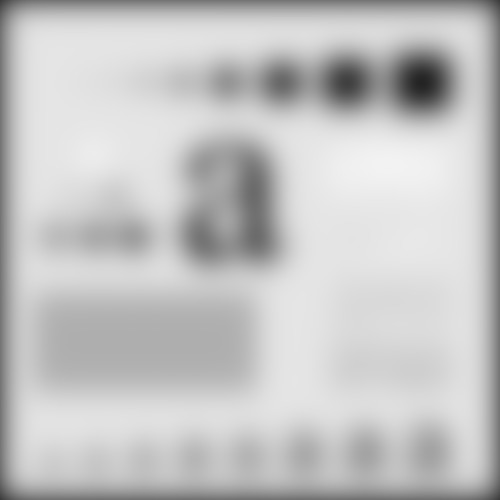
\includegraphics[width=0.3\textwidth]{pro3/GLPF/GLPF_10}&
		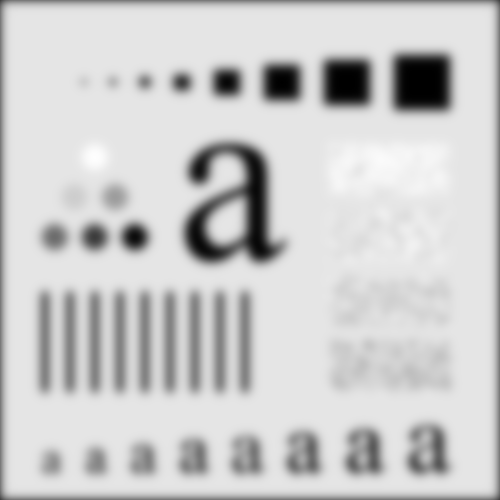
\includegraphics[width=0.3\textwidth]{pro3/GLPF/GLPF_30} \\
		original image &  $D_0=10$ &  $D_0=30$\\
		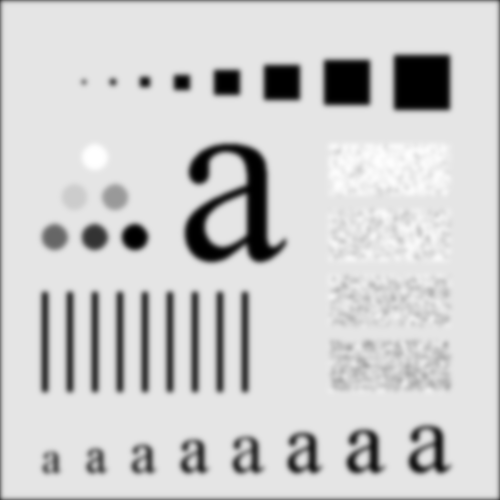
\includegraphics[width=0.3\textwidth]{pro3/GLPF/GLPF_60}&
		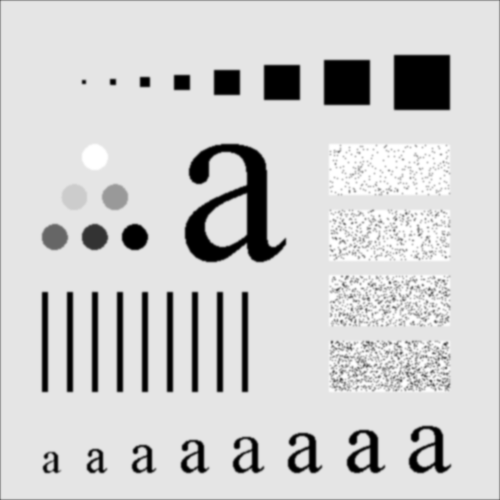
\includegraphics[width=0.3\textwidth]{pro3/GLPF/GLPF_160}&
		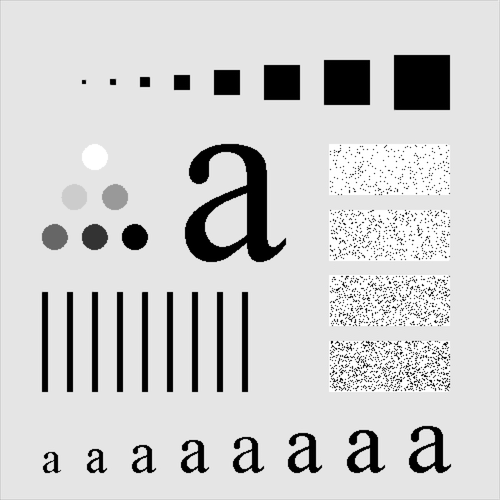
\includegraphics[width=0.3\textwidth]{pro3/GLPF/GLPF_460} \\
		 $D_0=60$ &  $D_0=160$ &  $D_0=460$
	\end{tabular}
	\caption{GLPF result of \textbf{characters\_test\_pattern.tif} in spatial domain}
	\label{pro3_fig3}
\end{figure}

\begin{figure}[!htbp]
	\centering
	\begin{tabular}{ccc} 
		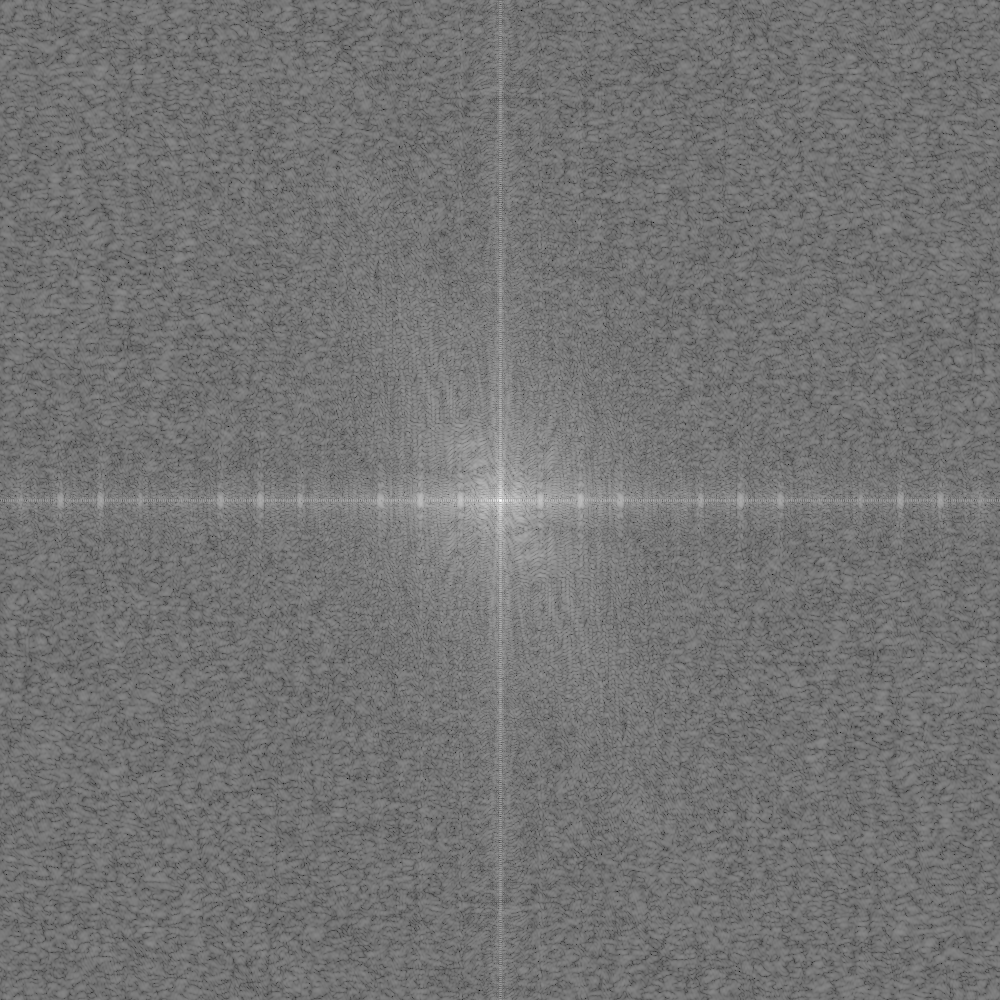
\includegraphics[width=0.3\textwidth]{pro3/org_spectrum}&
		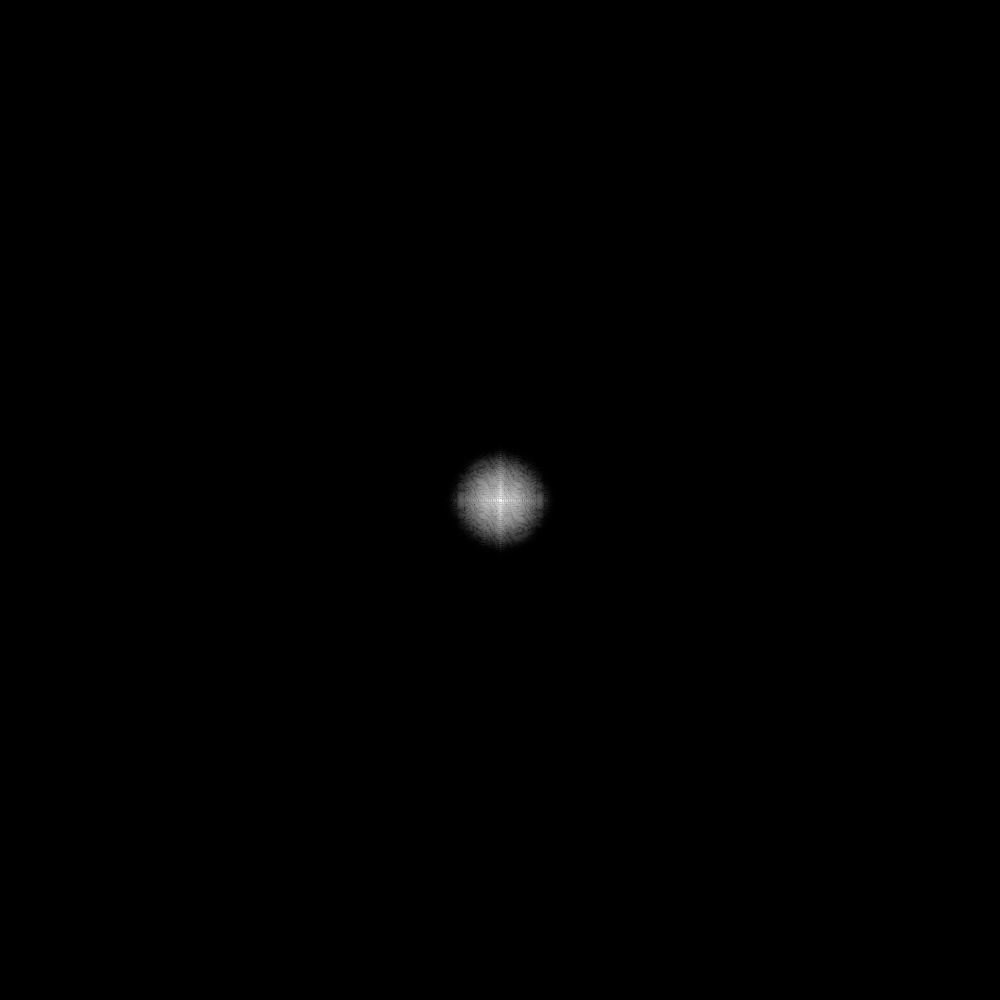
\includegraphics[width=0.3\textwidth]{pro3/GLPF/GLPF_10_spectrum}&
		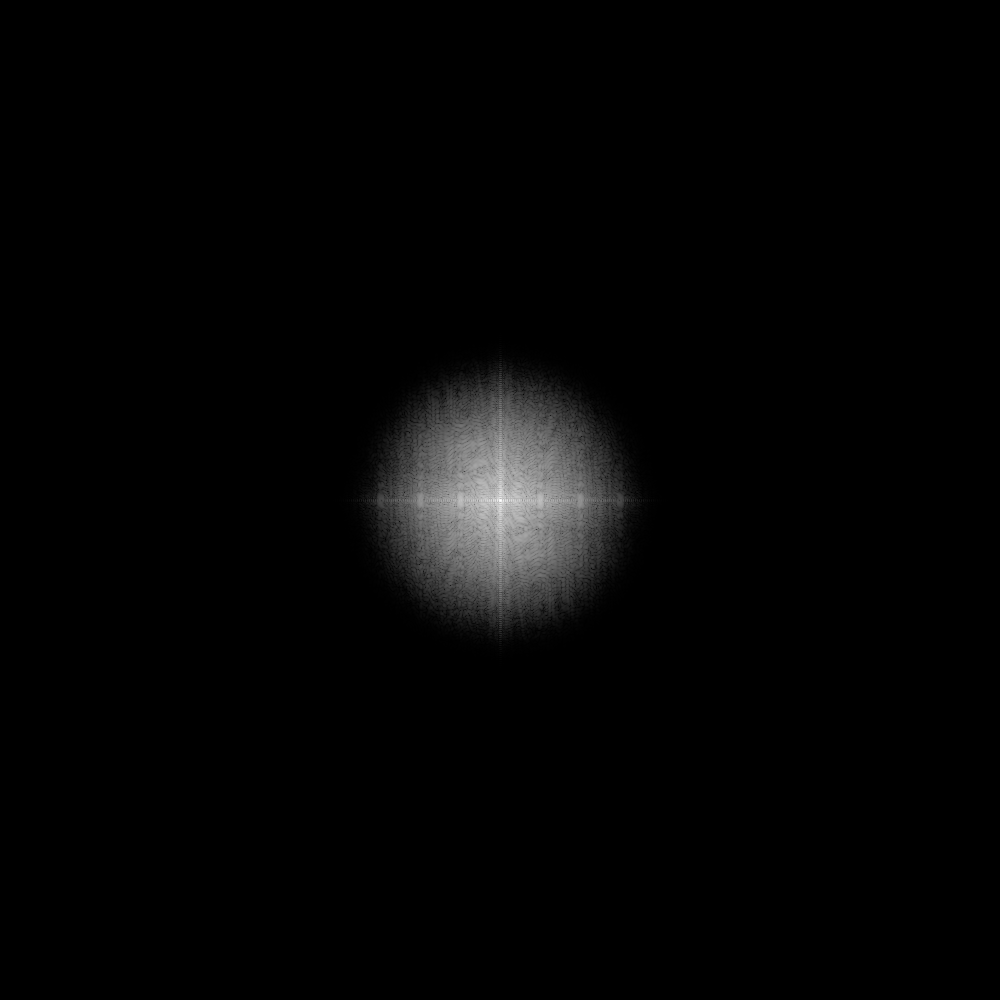
\includegraphics[width=0.3\textwidth]{pro3/GLPF/GLPF_30_spectrum} \\
		original image &  $D_0=10$ &  $D_0=30$\\
		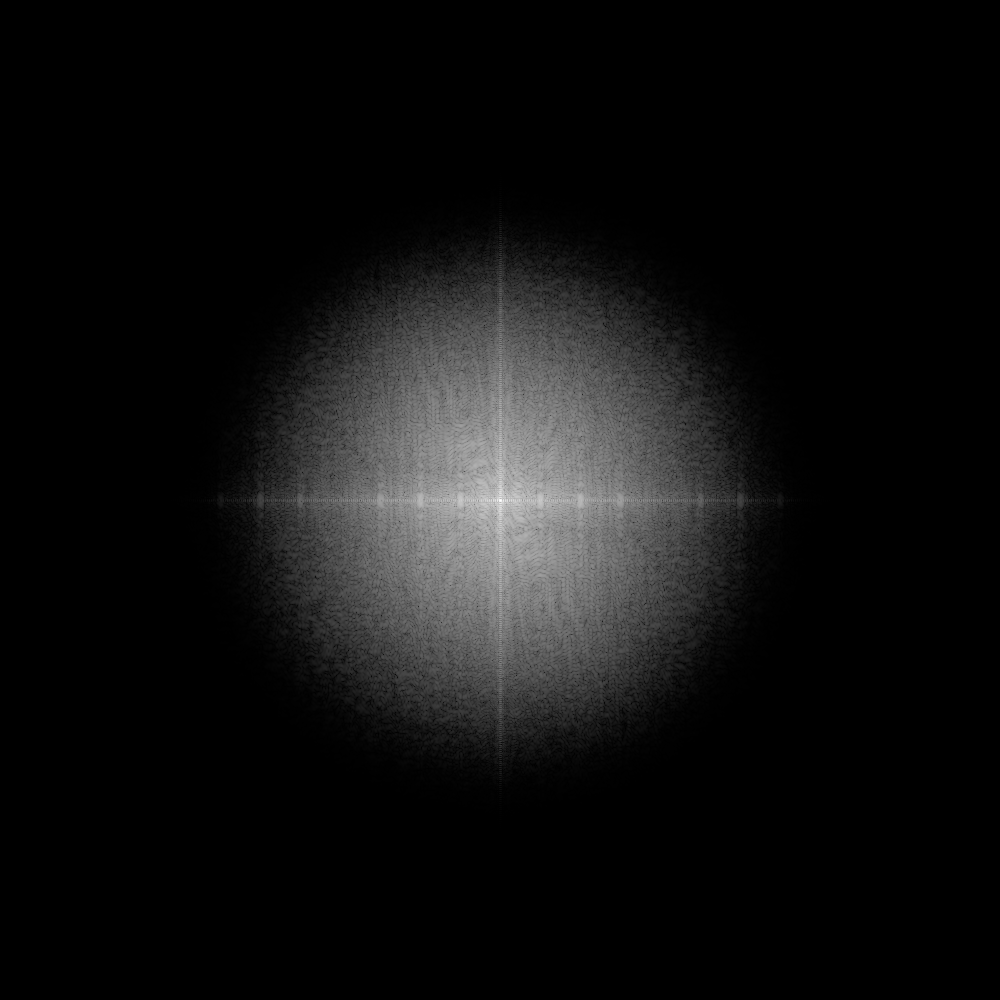
\includegraphics[width=0.3\textwidth]{pro3/GLPF/GLPF_60_spectrum}&
		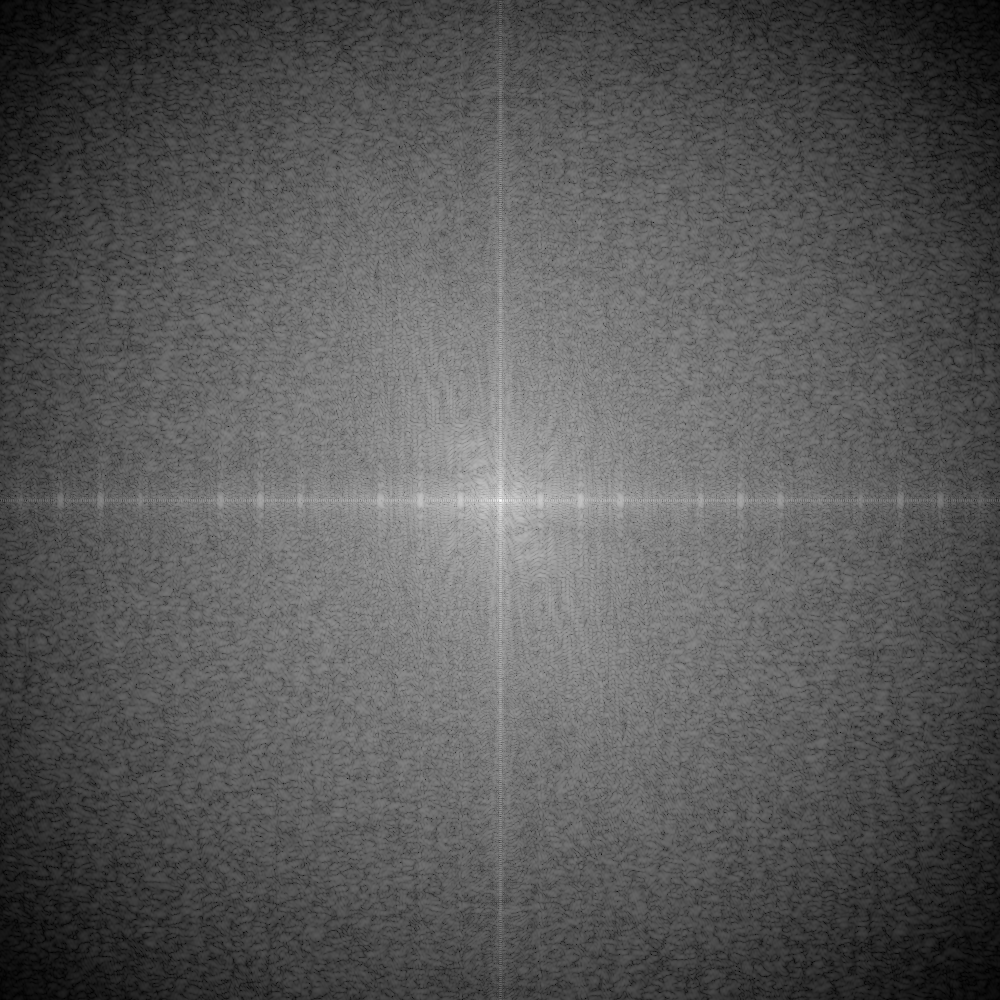
\includegraphics[width=0.3\textwidth]{pro3/GLPF/GLPF_160_spectrum}&
		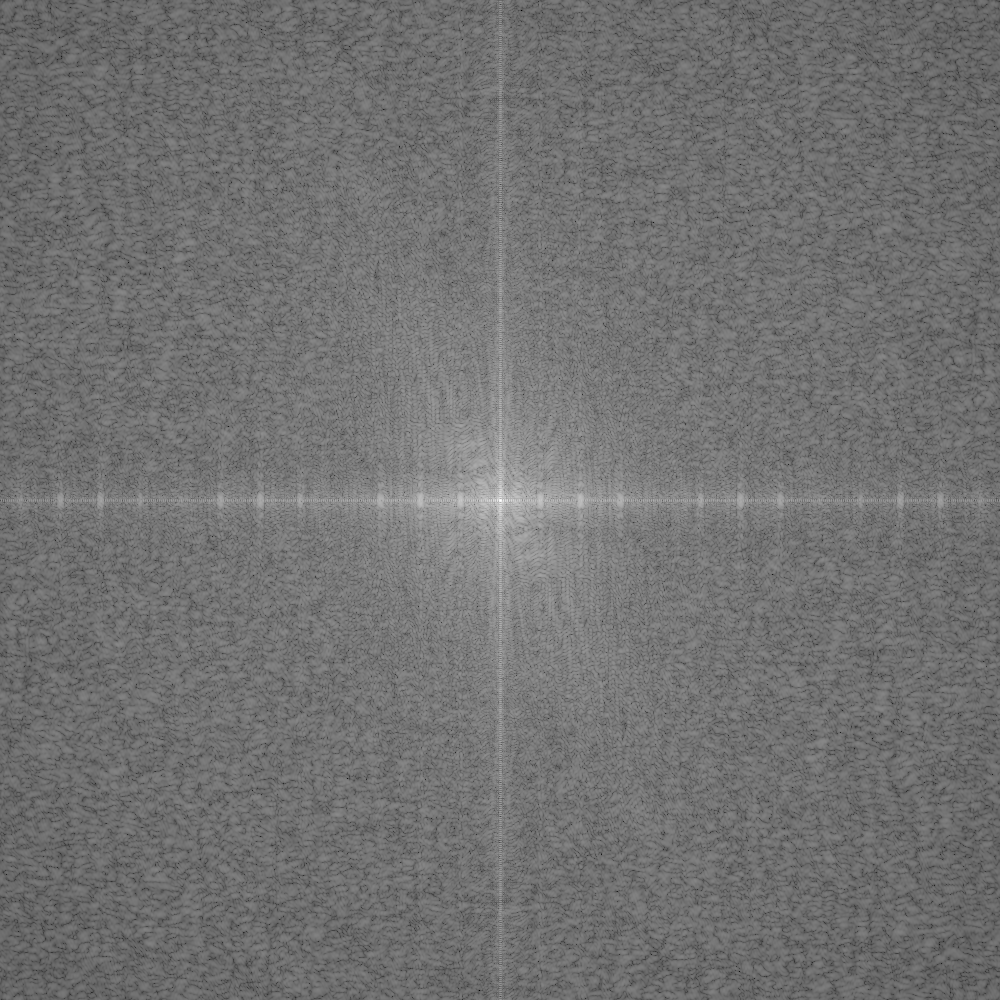
\includegraphics[width=0.3\textwidth]{pro3/GLPF/GLPF_460_spectrum} \\
		 $D_0=60$ &  $D_0=160$ &  $D_0=460$
	\end{tabular}
	\caption{GLPF result of \textbf{characters\_test\_pattern.tif} in frequency domain}
	\label{pro3_fig4}
\end{figure}

\begin{figure}[!htbp]
	\centering
	\begin{tabular}{ccc} 
		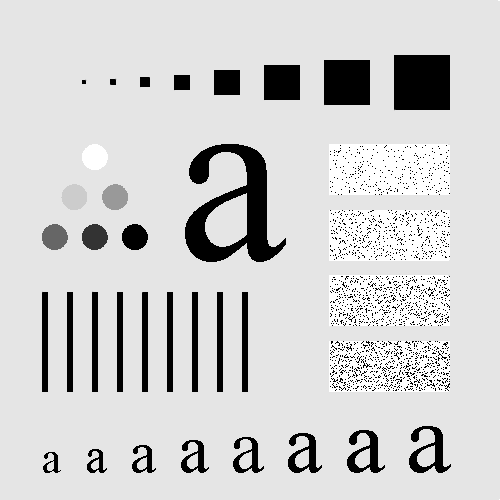
\includegraphics[width=0.3\textwidth]{pro3/org}&
		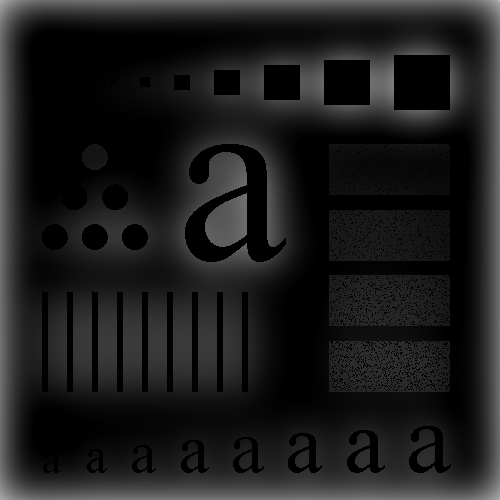
\includegraphics[width=0.3\textwidth]{pro3/BHPF/BHPF_10}&
		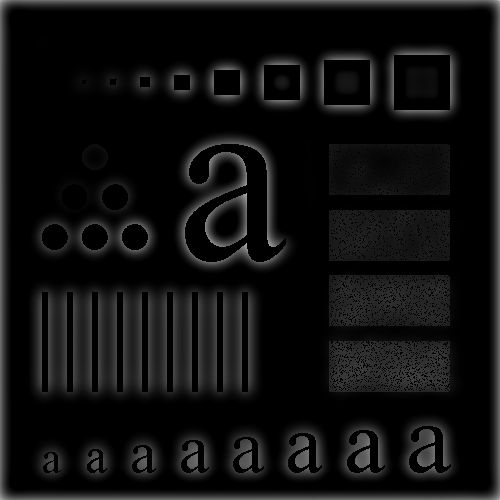
\includegraphics[width=0.3\textwidth]{pro3/BHPF/BHPF_30} \\
		original image &  $D_0=10$ &  $D_0=30$\\
		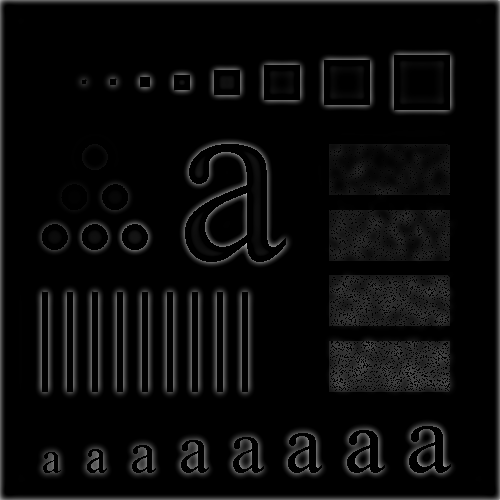
\includegraphics[width=0.3\textwidth]{pro3/BHPF/BHPF_60}&
		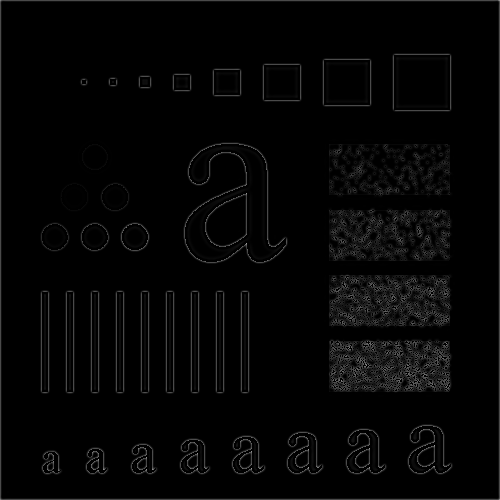
\includegraphics[width=0.3\textwidth]{pro3/BHPF/BHPF_160}&
		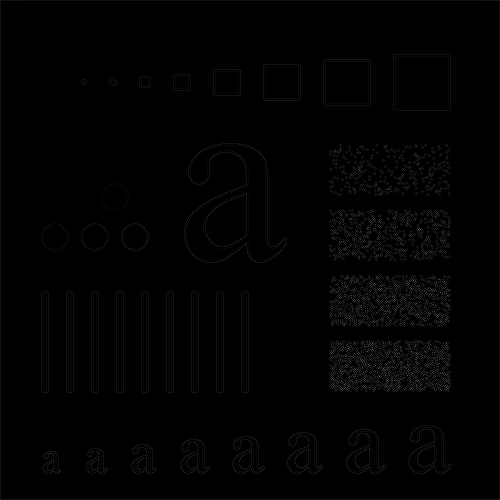
\includegraphics[width=0.3\textwidth]{pro3/BHPF/BHPF_460} \\
		 $D_0=60$ &  $D_0=160$ &  $D_0=460$
	\end{tabular}
	\caption{BHPF$(n=2)$ result of \textbf{characters\_test\_pattern.tif} in spatial domain}
	\label{pro3_fig5}
\end{figure}

\begin{figure}[!htbp]
	\centering
	\begin{tabular}{ccc} 
		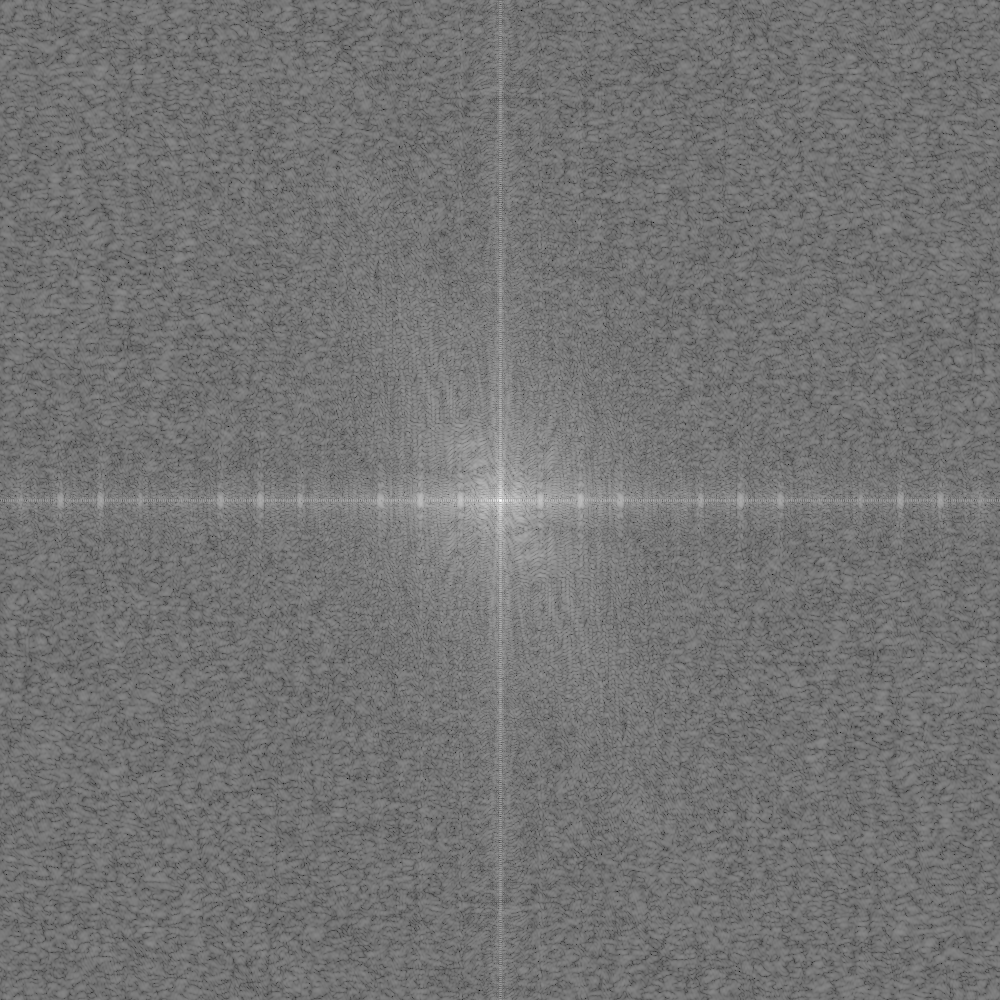
\includegraphics[width=0.3\textwidth]{pro3/org_spectrum}&
		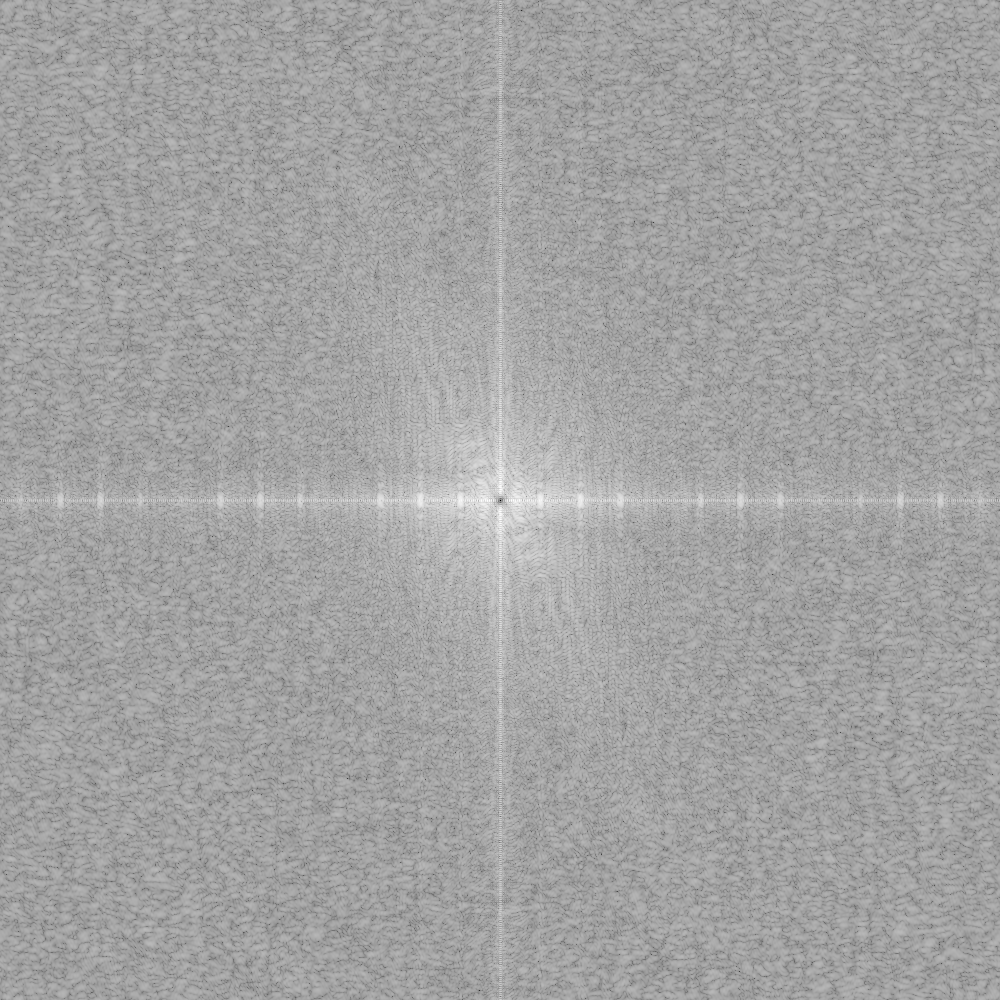
\includegraphics[width=0.3\textwidth]{pro3/BHPF/BHPF_10_spectrum}&
		\includegraphics[width=0.3\textwidth]{pro3/BHPF/BHPF_30_spectrum} \\
		original image &  $D_0=10$ &  $D_0=30$\\
		\includegraphics[width=0.3\textwidth]{pro3/BHPF/BHPF_60_spectrum}&
		\includegraphics[width=0.3\textwidth]{pro3/BHPF/BHPF_160_spectrum}&
		\includegraphics[width=0.3\textwidth]{pro3/BHPF/BHPF_460_spectrum} \\
		 $D_0=60$ &  $D_0=160$ &  $D_0=460$
	\end{tabular}
	\caption{BHPF$(n=2)$ result of \textbf{characters\_test\_pattern.tif} in frequency domain}
	\label{pro3_fig6}
\end{figure}

\section{Noise Generation and Reduction}
\subsection{Implementation}
This assignment requires us to generate noise which yield different distribution 
function. We need to figure out how to produce a random variable with different
distribution function from a uniform random variable. I consulted \cite{randomv}
to find a way.

The common way is to calculate a random variable as follows:
\begin{equation}
	X=F_X^{-1}(U)
\end{equation}
where $U$ is a uniform random variable and $F_x$ is the cumulative distribution 
function of our target random variable $X$. Take exponential random variable as 
an example, its CDF is $F_X=1-e^{-x/a},x\geq 0$ and then we get $x=-\frac{1}{a}ln(1-u)$,
where $us$ is a uniform random variable and $x$ is our target variable.
For rayleigh, things are quite similar. 

However, we cannot get the CDF of Gaussian random variable, but I found it has a formula
\begin{equation}
	F(x)=\Phi (\frac{x-\mu}{\sigma})=\frac{1}{2}\left[1+\textrm{erf}\left(\frac{x-\mu}{\sigma\sqrt{2}}\right)\right]
\end{equation}
where $\textrm{erf}(x)=\frac{2}{\sqrt{2}}\int_{0}^{x} e^{-t^2} dt$. This function is 
built in matlab, and then we can easily implement gaussian noise.
However, this is not the only way I found, a usual way we used is 
an algorithm called Box-Muller method. I have tried this and the distribution
is a little different with the one created by the built-in function \textbf{randn}.
Thus, we choose the first way.

Gamma random variable is defined as the sum of $b$ indenpendent exponential random
variable $Y_i$, each with mean $1/a$. We can use the sum of exponential random variable
to generate a Gamma random variable, or we can use uniform variables to generate them directly, 
which can provide a little acceleration.

Other part of this assignment are just implemented as the textbook instructed, so we won't talk more about
the details.

\subsection{Result Analysis}

After running the script \textbf{testdemo.m}, you will get the following results.
Only part of 
results are presented here, you can browse all results by running \textbf{testdemo.m} or
look into the file folder \textbf{./outputs/pro4}.

As shown in Figure \ref{pro4_fig1} and \ref{pro4_fig2}, our noise generator works well.
To get the similar apperance to \textbf{FIGURE 5.4} in our textbook, I adjusts the parameters
carefully and plot the histogram in a proper range, which is not always [0,255]. This is because
some value will extends that range, thus we need to enlarge our display range to see
its full apperance.

Figure \ref{pro4_fig3} presents the result of different kinds of filters applied to
an image corrupted with both uniform and pepper\&salt noise. As expected,
the arithmetic and geometric mean filters (especially the latter) did not do
well because of the presence of impulse noise. The median and alpha-trimmed
filters performed much better, with the alpha-trimmed filter giving slightly better
noise reduction. You can compare with these results with those presented as
\textbf{FIGURE 5.12} in the textbook. Most of the results are similar, but there are 
some difference between the two results of geometric filter.

\begin{figure}[!htbp]
	\centering
	\begin{tabular}{ccc} 
		\includegraphics[width=0.3\textwidth]{pro4/gaussian}&
		\includegraphics[width=0.3\textwidth]{pro4/rayleigh}&
		\includegraphics[width=0.3\textwidth]{pro4/gamma} \\
		Gaussian noise(a=-0.1,b=0.1) &  Rayleigh noise(a=-0.3,b=0.04) &  Gamma noise(a=15,b=2)\\
		\includegraphics[width=0.3\textwidth]{pro4/gaussianHist}&
		\includegraphics[width=0.3\textwidth]{pro4/rayleighHist}&
		\includegraphics[width=0.3\textwidth]{pro4/gammaHist} \\
		 Histogram of Gaussian noise &  Histogram of Rayleigh noise &  Histogram of Gamma noise
	\end{tabular}
	\caption{Noise generation 1}
	\label{pro4_fig1}
\end{figure}

\begin{figure}[!htbp]
	\centering
	\begin{tabular}{ccc} 
		\includegraphics[width=0.3\textwidth]{pro4/exponential}&
		\includegraphics[width=0.3\textwidth]{pro4/uniform}&
		\includegraphics[width=0.3\textwidth]{pro4/impulse} \\
		Exponential noise(a=15) &  Uniform noise(a=-0.1,b=0.2) &  Impulse noise(a=0.05,b=0.05)\\
		\includegraphics[width=0.3\textwidth]{pro4/exponentialHist}&
		\includegraphics[width=0.3\textwidth]{pro4/uniformHist}&
		\includegraphics[width=0.3\textwidth]{pro4/impulseHist} \\
		 Histogram of Exponential noise &  Histogram of Uniform noise &  Histogram of Impulse noise
	\end{tabular}
	\caption{Noise generation 2}
	\label{pro4_fig2}
\end{figure}

\begin{figure}[!htbp]
	\centering
	\begin{tabular}{ccc} 
		\includegraphics[width=0.3\textwidth]{pro4/5_12_a}&
		\includegraphics[width=0.3\textwidth]{pro4/5_12_b}&
		\includegraphics[width=0.3\textwidth]{pro4/5_12_c} \\
		uniform noise &  uniform and pepper\&sale noise &  $5\times 5$ arithmetic mean filter\\
		\includegraphics[width=0.3\textwidth]{pro4/5_12_d}&
		\includegraphics[width=0.3\textwidth]{pro4/5_12_e}&
		\includegraphics[width=0.3\textwidth]{pro4/5_12_f} \\
		$5\times 5$ geometric mean filter &  $5\times 5$ median filter & $5\times 5$ alpha-trimmed filter(d=10)
	\end{tabular}
	\caption{Comparison between different noise reduction mothods}
	\label{pro4_fig3}
\end{figure}

\newpage
\section{Image restoration}
\subsection{Implementation}
In this assignment, I continue using the DFT and IDFT function \textbf{dip2DDFT.m} and 
\textbf{dip2DIDFT.m} which implemented in assignment 3. And follow the same steps
of frequency filtering as mentioned in section 3.
However, to get similar result as \textbf{FIGURE 5.26} in textbook presented, we need to circular pad 
the image itself, \emph{s.t.}, we invoke built-in function \textbf{repmat} to repeat 
the original image 4 times. 

For the implementation inverse filter, it will be a problem when there appears zeros
or quite small values in the degradation function $H$. To avoid this, the textbook introduce
frequency lowpass filter to reduce
the probability of encountering zero values. However, this is not a stable solution and it doesn't 
work when trying to restore our motion blurred image.
The way here I used is adopted from \cite{inversef}. Now the inverse function is not
always $1/H$, when it is too high, the value will be abandoned. That is,
\begin{equation}
	H^*(x)=\left\{\begin{array}{ll}\frac{1}{H(x)},&H(x)\geq a\\
	0,&H(x)<a\end{array}\right.
\end{equation}
where $H^*$ is inverse filter function. The threshold $a$ here in this implementation is set to be $10^{-10}$.
Finally, I found that if we use threshold way and lowpass filter simultaneously,
we will get a very good restoration.

For better comparison, the value $K$ in equation 
\begin{equation}
	\hat{F}(u,v)=\left[\frac{1}{H(u,v)}\frac{|H(u,v)|^2}{|H(u,v)|^2+K}\right]G(u,v)
\end{equation}
is calculated as $K=1/\textrm{SNR}$.

\subsection{Result Analysis}
After running the script \textbf{testdemo.m}, you will get the following result. 

As show in Figure \ref{pro5_fig1},  our result is similar to those presented as 
\textbf{FIGURE 5.26} in our textbook. However, the parameters are different to get
similar result, which are displayed in their caption. Thus, for the rest part of this assignment, 
we will use $a=b=0.05,T=1$ to get our motion blurred image.

Results shown in Figure \ref{pro5_fig2} can be a little different with \textbf{FIGURE 5.29}
in our textbook. This can be caused by using threshold way to implement the inverse filter.
Additionly, in the fourth column of the result figure, you can see that using inverse filter with
threshold and lowpass filter simultaneously will get a better result than using inverse filter
directly.

\begin{figure}[!htbp]
	\centering
	\begin{tabular}{ccc} 
		\includegraphics[width=0.3\textwidth]{pro5/5_26_a}&
		\includegraphics[width=0.3\textwidth]{pro5/5_26_a_b}&
		\includegraphics[width=0.3\textwidth]{pro5/5_26_b} \\
		Original image &  Blurred Image(a,b=0.1,T=1) &  Blurred Image(a,b=0.05,T=1)
	\end{tabular}
	\caption{Motion blur}
	\label{pro5_fig1}
\end{figure}

\begin{figure}[!htbp]
	\centering
	\begin{tabular}{cccc} 
		\includegraphics[width=0.2\textwidth]{pro5/5_29_a}&
		\includegraphics[width=0.2\textwidth]{pro5/5_29_b}&
		\includegraphics[width=0.2\textwidth]{pro5/5_29_c}&
		\includegraphics[width=0.2\textwidth]{pro5/5_29_b+}\\
		$\mu=0,\sigma^2=650$ &  inverse filter &  Winner filter & inverse+lowpass filter\\
		\includegraphics[width=0.2\textwidth]{pro5/5_29_d}&
		\includegraphics[width=0.2\textwidth]{pro5/5_29_e}&
		\includegraphics[width=0.2\textwidth]{pro5/5_29_f}&
		\includegraphics[width=0.2\textwidth]{pro5/5_29_e+}\\
		$\mu=0,\sigma^2=65$ &  inverse filter &  Winner filter & inverse+lowpass filter\\
		\includegraphics[width=0.2\textwidth]{pro5/5_29_g}&
		\includegraphics[width=0.2\textwidth]{pro5/5_29_h}&
		\includegraphics[width=0.2\textwidth]{pro5/5_29_i}&
		\includegraphics[width=0.2\textwidth]{pro5/5_29_h+}\\
		$\mu=0,\sigma^2=0.0065$ &  inverse filter &  Winner filter & inverse+lowpass filter\\
	\end{tabular}
	\caption{Restoration with inverse and Winner filter}
	\label{pro5_fig2}
\end{figure}

\section{Geometric transform}
After running the script \textbf{testdemo.m}, you will get the following result.

These results shows that our implementation has a good compatibility. The rotation 
can be applied around different center point and with different angles. Translate 
with different shift value can all be satisfied. Scaling of image can enlarge or shrink 
the original image or even flip it with a nagative paramter specified. For ratating 
and translating, you can choose 3 types of padding, which are padding black, white and images.

By constrasting with two images in Figure \ref{pro6_fig3},\ref{pro6_fig5} and \ref{pro6_fig7},
especially the first one and the third one, you can see difference between near neighbor interpolation 
and Bilinear interpolation. The former will appear more coarse and artificiial while the latter
will get smoother result.

\begin{figure}[!htbp]
	\centering
	\begin{tabular}{cccc} 
		\includegraphics[width=0.2\textwidth]{pro6/rotate/originRotate}&
		\includegraphics[width=0.2\textwidth]{pro6/rotate/rotate_30_black}&
		\includegraphics[width=0.2\textwidth]{pro6/rotate/rotate_30_white}&
		\includegraphics[width=0.2\textwidth]{pro6/rotate/rotate_30_image}\\
		Original image & Black padded& White padded & Image padded
	\end{tabular}
	\caption{Rotate with different paddings}
	\label{pro6_fig1}
\end{figure}

\begin{figure}[!htbp]
	\centering
	\begin{tabular}{ccc} 
		\includegraphics[width=0.3\textwidth]{pro6/rotate/rotate_30_leftc}&
		\includegraphics[width=0.3\textwidth]{pro6/rotate/rotate_60_center}&
		\includegraphics[width=0.3\textwidth]{pro6/rotate/rotate_-45_rightc}\\
		$c=(0,0),\alpha=30^{\circ}$ &$c=(M/2,N/2),\alpha=60^{\circ}$ & $c=(M-1,N-1),\alpha=-45^{\circ}$
	\end{tabular}
	\caption{Rotate with different center points and angles}
	\label{pro6_fig2}
\end{figure}

\begin{figure}[!htbp]
	\centering
	\begin{tabular}{cccc} 
		\includegraphics[width=0.23\textwidth]{pro6/translate/originTrans}&
		\includegraphics[width=0.23\textwidth]{pro6/translate/trans_30_30_black}&
		\includegraphics[width=0.23\textwidth]{pro6/translate/trans_-30_5_40_3_white}&
		\includegraphics[width=0.23\textwidth]{pro6/translate/trans_80_40_image}\\
		Original image & Black+(30,30)&White(-30.5,40.3) & Image+(80,40)
	\end{tabular}
	\caption{Translate image with different pad type and displacement}
	\label{pro6_fig4}
\end{figure}

\begin{figure}[!htbp]
	\centering
	\begin{tabular}{cc}
	\includegraphics[scale=0.3]{pro6/scale/originScale}&
	\includegraphics[scale=0.3]{pro6/scale/scale_0_5_0_5}\\
	Original image& $\times [0.5,0.5]$\\
	\includegraphics[scale=0.3]{pro6/scale/scale_1_5_1_5}&
	\includegraphics[scale=0.3]{pro6/scale/scale_1_-1}\\
	$\times [1.5,1.5]$& $\times [1,-1]$
	\end{tabular}
	\caption{Scale image with different enlarge parameters}
	\label{pro6_fig6}
\end{figure}

\begin{figure}[!htbp]
	\centering
	\begin{tabular}{cc} 
		\includegraphics[width=0.4\textwidth]{pro6/rotate/rotate_nn}&
		\includegraphics[width=0.4\textwidth]{pro6/rotate/rotate_bilinear}\\
		Nearest neighbor &Bilinear 
	\end{tabular}
	\caption{Rotate with different interpolation methods}
	\label{pro6_fig3}
\end{figure}

\begin{figure}[!htbp]
	\centering
	\begin{tabular}{cc} 
		\includegraphics[width=0.45\textwidth]{pro6/translate/translate_nn}&
		\includegraphics[width=0.45\textwidth]{pro6/translate/translate_bilinear}\\
		Nearest neighbor &Bilinear 
	\end{tabular}
	\caption{Translate with different interpolation methods}
	\label{pro6_fig5}
\end{figure}

\begin{figure}[!htbp]
	\centering
	\begin{tabular}{cc} 
		\includegraphics[width=0.45\textwidth]{pro6/scale/scale_nn}&
		\includegraphics[width=0.45\textwidth]{pro6/scale/scale_bilinear}\\
		Nearest neighbor &Bilinear 
	\end{tabular}
	\caption{Scale with different interpolation methods}
	\label{pro6_fig7}
\end{figure}

\section{Transform image compression}
After running the script \textbf{testdemo.m}, you will get the following result.

Figure \ref{pro7_fig1} shows the result of DCT compression using zonal mask
and \ref{pro7_fig2},\ref{pro7_fig3} display the result of same compression with different threshold
masks. The threshold mask way is implemented with normalization array.
You can easily find that a larger normalization array will get a lower quality image.
The implementation of DCT is similar to the DFT in a vectorize way.

The result of DWT compression with different wavelets are displayed in Figure \ref{pro7_fig4}.
The implementation of DWT is fast discrete wavelet transform as the textbook instructs.
I use the built-in function \textbf{conv2} to speed up the whole process, since the convolution implementation
is not the critical part of this assignment.

\begin{figure}[!htbp]
	\centering
	\begin{tabular}{ccc} 
		\includegraphics[width=0.3\textwidth]{pro7/dct/8_31_a}&
		\includegraphics[width=0.3\textwidth]{pro7/dct/8_31_b}&
		\includegraphics[width=0.3\textwidth]{pro7/dct/8_31_c}\\
		 $\mathbf{Z}$& $\mathbf{2Z}$ & $\mathbf{3Z}$\\
		\includegraphics[width=0.3\textwidth]{pro7/dct/8_31_d}&
		\includegraphics[width=0.3\textwidth]{pro7/dct/8_31_e}&
		\includegraphics[width=0.3\textwidth]{pro7/dct/8_31_f}\\
		$\mathbf{4Z}$& $\mathbf{5Z}$ & $\mathbf{6Z}$
	\end{tabular}
	\caption{DCT compression using Threshold mask(with normalization array)}
	\label{pro7_fig2}
\end{figure}

\begin{figure}[!htbp]
	\centering
	\begin{tabular}{ccc} 
		\includegraphics[width=0.3\textwidth]{pro7/dct/8_31_a_diff}&
		\includegraphics[width=0.3\textwidth]{pro7/dct/8_31_b_diff}&
		\includegraphics[width=0.3\textwidth]{pro7/dct/8_31_c_diff}\\
		 $\mathbf{Z}$& $\mathbf{2Z}$ & $\mathbf{3Z}$\\
		\includegraphics[width=0.3\textwidth]{pro7/dct/8_31_d_diff}&
		\includegraphics[width=0.3\textwidth]{pro7/dct/8_31_e_diff}&
		\includegraphics[width=0.3\textwidth]{pro7/dct/8_31_f_diff}\\
		$\mathbf{4Z}$& $\mathbf{5Z}$ & $\mathbf{6Z}$
	\end{tabular}
	\caption{Difference images using Threshold mask(with normalization array)}
	\label{pro7_fig3}
\end{figure}

\begin{figure}[!htbp]
	\centering
	\begin{tabular}{ccc} 
		\includegraphics[width=0.25\textwidth]{pro7/origin}&
		\includegraphics[width=0.25\textwidth]{pro7/dct/zonal}&
		\includegraphics[width=0.25\textwidth]{pro7/dct/zonal_diff}\\
		 Original image& Reconstructed image & difference image
	\end{tabular}
	\caption{DCT compression using zonal mask}
	\label{pro7_fig1}
\end{figure}

\begin{figure}[!htbp]
	\centering
	\begin{tabular}{cccc} 
		\includegraphics[width=0.18\textwidth]{pro7/dwt/haar_res}&
		\includegraphics[width=0.18\textwidth]{pro7/dwt/db_res}&
		\includegraphics[width=0.18\textwidth]{pro7/dwt/sym_res}&
		\includegraphics[width=0.18\textwidth]{pro7/dwt/cdf_res}\\
		 Haar & Daubechies & Symlet &CDF\\
		\multicolumn{2}{c}{
			\includegraphics[width=0.38\textwidth]{pro7/dwt/haar_dwt}
		}&
		\multicolumn{2}{c}{
			\includegraphics[width=0.38\textwidth]{pro7/dwt/db_dwt}
		}\\
		\multicolumn{2}{c}{
			DWT using Haar
		}&
		\multicolumn{2}{c}{
			DWT using Daubechies
		}\\
		\multicolumn{2}{c}{
			\includegraphics[width=0.38\textwidth]{pro7/dwt/sym_dwt}
		}&
		\multicolumn{2}{c}{
			\includegraphics[width=0.38\textwidth]{pro7/dwt/cdf_dwt}
		}\\
		\multicolumn{2}{c}{
			DWT using Symlet
		}&
		\multicolumn{2}{c}{
			DWT using Cohen-Daubechies-Feauveau
		}
	\end{tabular}
	\caption{DWT compression with different wavelets}
	\label{pro7_fig4}
\end{figure}

\newpage
\newpage
\section{Morpholigical Processing}
\subsection{implementation}
The critical part of this assignment is reconstruction with geodesic dilation.
To accelerate the reconstruction process, I implement this reconstruction function 
as \cite{vincent} instructs. You can learn about more details in this article.

\subsection{Result Analysis}
After running the script \textbf{testdemo.m}, you will get the following result.

Figure \ref{pro8_fig1},\ref{pro8_fig2} and \ref{pro8_fig3} shows the result of opening by reconstruction,
filling holes and border clearing. These results are exactly the same as \textbf{FIGURE 9.29},\textbf{9.31} and
\textbf{9.32} in the textbook.

\begin{figure}[!htbp]
	\centering
	\begin{tabular}{cc} 
		\includegraphics[width=0.45\textwidth]{pro8/9_29_a}&
		\includegraphics[width=0.45\textwidth]{pro8/9_29_b}\\
		Original image &Erosion with SE size is $51\times 1$ \\
		\includegraphics[width=0.45\textwidth]{pro8/9_29_c}&
		\includegraphics[width=0.45\textwidth]{pro8/9_29_d}\\
		Opening of original image with same size SE & Result of opening by reconstruction
	\end{tabular}
	\caption{Opening by reconstruction}
	\label{pro8_fig1}
\end{figure}

\begin{figure}[!htbp]
	\centering
	\begin{tabular}{cc} 
		\includegraphics[width=0.45\textwidth]{pro8/9_31_a}&
		\includegraphics[width=0.45\textwidth]{pro8/9_31_b}\\
		Original image &Complement of original image \\
		\includegraphics[width=0.45\textwidth]{pro8/9_31_c}&
		\includegraphics[width=0.45\textwidth]{pro8/9_31_d}\\
		Marker image & Result of hole-filling
	\end{tabular}
	\caption{Filling holes}
	\label{pro8_fig2}
\end{figure}

\begin{figure}[!htbp]
	\centering
	\begin{tabular}{cc} 
		\includegraphics[width=0.45\textwidth]{pro8/9_32_a}&
		\includegraphics[width=0.45\textwidth]{pro8/9_32_b}\\
		Marker image &Result of border clearing
	\end{tabular}
	\caption{Border clearing}
	\label{pro8_fig3}
\end{figure}

\section{Image segmentation}
\subsection{Implementation}
The critical part of the first task in this assignment is to implement Marr-Hildreth edge
detector and canny detector. The first one can be directly implemented as our textbook
instructs. However, our textbook doesn't introduce clearly about the edge connection process
in canny detector. This process is kind of similar to the BFS process. The difference is that 
we can only choose strong edge pixels as start point. For more details, you can consult the comments
in my codes.

The second task thresholding is a easy task. To implement the basic global thresholding, we need to
find the point which divide the intensity to two parts with same average intensity. This goal can be
achieved by operating the histogram without iteration. The Otsu's way can be directly implemented as
our textbook tells.

\subsection{Result Analysis}
After running the script \textbf{testdemo.m}, you will get the following result.

Figure \ref{pro9_fig1} shows the comparison between different edge detectors and 
and \ref{pro9_fig2} dipslays the result of two kinds of thresholding.
You can compare these two figures with \textbf{FIGURE 10.25} and \textbf{10.39} in the
textbook, the similarity between
them will announce the correctness of our results.

\begin{figure}[!htbp]
	\centering
	\begin{tabular}{ccc} 
		\includegraphics[width=0.3\textwidth]{pro9/10_25_a}&
		\includegraphics[width=0.3\textwidth]{pro9/10_25_c}&
		\includegraphics[width=0.3\textwidth]{pro9/10_25_d}\\
		 Origin image scaled to [0,1]& the Marr-Hidreth algorithm  & the Canny algorithm\\
		\includegraphics[width=0.3\textwidth]{pro9/10_25_roberts}&
		\includegraphics[width=0.3\textwidth]{pro9/10_25_prewitt}&
		\includegraphics[width=0.3\textwidth]{pro9/10_25_b}\\
		$5\times 5$ average filter+Roberts mask& $5\times 5$ average filter+Prewitt mask & $5\times 5$ average filter+Sobel mask
	\end{tabular}
	\caption{Comparison between different edge detectors}
	\label{pro9_fig1}
\end{figure}

\begin{figure}[!htbp]
	\centering
	\begin{tabular}{cc} 
		\includegraphics[width=0.45\textwidth]{pro9/10_39_a}&
		\includegraphics[width=0.45\textwidth]{pro9/10_39_b}\\
		Original image &Histogram of original image \\
		\includegraphics[width=0.45\textwidth]{pro9/10_39_c}&
		\includegraphics[width=0.45\textwidth]{pro9/10_39_d}\\
		Basic global algorithm$(T=170,\eta=0.1987)$ & Otsu's method$(T=181,\eta=0.2174)$
	\end{tabular}
	\caption{Thresholding}
	\label{pro9_fig2}
\end{figure}

\section{Image representation and description}
After running the script \textbf{testdemo.m}, you will get the following result.

\begin{shaded}
	\noindent For image noisy\_stroke.tif:\\
	Default 8-directional chain code start with (2,5):\\
	0 0 0 0 6 0 6 6 6 6 6 6 6 6 4 4 4 4 4 4 2 4 2 2 2 2 2 0 2 2 0 2\\
	and its first difference is:\\
	0 0 0 6 2 6 0 0 0 0 0 0 0 6 0 0 0 0 0 6 2 6 0 0 0 0 6 2 0 6 2 6\\
	 Normalized 8-directional chain code starts with (2,5), its value is:\\
	0 0 0 0 6 0 6 6 6 6 6 6 6 6 4 4 4 4 4 4 2 4 2 2 2 2 2 0 2 2 0 2\\
	and its first difference is:\\
	0 0 0 6 2 6 0 0 0 0 0 0 0 6 0 0 0 0 0 6 2 6 0 0 0 0 6 2 0 6 2 6\\
	Eigenvalues of the covariance matrices obtained from all 6 images:\\
	lambda\_1=10344.304804\\
	lambda\_2=2965.897734\\
	lambda\_3=1400.635021\\
	lambda\_4=203.455480\\
	lambda\_5=94.277394\\
	lambda\_6=31.037280
\end{shaded}

The process of getting Freeman chaincode is shown in Figure \ref{pro10_fig1}.
The chaincode are output as vectors and displayed in the frame above.
Figure \ref{pro10_fig2},\ref{pro10_fig3},\ref{pro10_fig4},\ref{pro10_fig5} shows the
the result of principal components analysis.

You can compare these figures with \textbf{FIGURE 11.5}, \textbf{11.38}, \textbf{11.39}, \textbf{11.41}
and \textbf{11.42} in the
textbook. Most of them are similar to each other. However, images in 
Figure \ref{pro10_fig5} is much differnet from the images in \textbf{FIGURE 11.42} in our textbook.
This may be caused by the different use of scaling way. But these images are similar to the images in 
\textbf{FIGURE 12.33} in the book \emph{DIP Using Matlab}.

\begin{figure}[!b]
	\centering
	\begin{tabular}{ccc} 
		\includegraphics[width=0.3\textwidth]{pro10/chaincode/11_5_a}&
		\includegraphics[width=0.3\textwidth]{pro10/chaincode/11_5_b}&
		\includegraphics[width=0.3\textwidth]{pro10/chaincode/11_5_c}\\
		 Original image & $9\times 9$ averaging filter  & thresholded using Otsu's method\\
		\includegraphics[width=0.3\textwidth]{pro10/chaincode/11_5_d}&
		\includegraphics[width=0.3\textwidth]{pro10/chaincode/11_5_e}&
		\includegraphics[width=0.3\textwidth]{pro10/chaincode/11_5_f}\\
		Boundary following & Subsample boundary(scale 50)& Connected resampled boundary
	\end{tabular}
	\caption{Freeman chaincode}
	\label{pro10_fig1}
\end{figure}

\begin{figure}[!htbp]
	\centering
	\begin{tabular}{ccc} 
		\includegraphics[width=0.3\textwidth]{pro10/PC/11_38_a}&
		\includegraphics[width=0.3\textwidth]{pro10/PC/11_38_b}&
		\includegraphics[width=0.3\textwidth]{pro10/PC/11_38_c}\\
		 Visible blue & visible green  & visible red\\
		\includegraphics[width=0.3\textwidth]{pro10/PC/11_38_d}&
		\includegraphics[width=0.3\textwidth]{pro10/PC/11_38_e}&
		\includegraphics[width=0.3\textwidth]{pro10/PC/11_38_f}\\
		near infrared & middle infrared& thermal infrared bands
	\end{tabular}
	\caption{Original multispectral images}
	\label{pro10_fig2}
\end{figure}

\begin{figure}[!htbp]
	\centering
	\begin{tabular}{ccc} 
		\includegraphics[width=0.3\textwidth]{pro10/PC/11_40_a}&
		\includegraphics[width=0.3\textwidth]{pro10/PC/11_40_b}&
		\includegraphics[width=0.3\textwidth]{pro10/PC/11_40_c}\\
		 Visible blue & visible green  & visible red\\
		\includegraphics[width=0.3\textwidth]{pro10/PC/11_40_d}&
		\includegraphics[width=0.3\textwidth]{pro10/PC/11_40_e}&
		\includegraphics[width=0.3\textwidth]{pro10/PC/11_40_f}\\
		near infrared & middle infrared& thermal infrared bands
	\end{tabular}
	\caption{Principal component images}
	\label{pro10_fig3}
\end{figure}

\begin{figure}[!htbp]
	\centering
	\begin{tabular}{ccc} 
		\includegraphics[width=0.3\textwidth]{pro10/PC/11_41_a}&
		\includegraphics[width=0.3\textwidth]{pro10/PC/11_41_b}&
		\includegraphics[width=0.3\textwidth]{pro10/PC/11_41_c}\\
		 Visible blue & visible green  & visible red\\
		\includegraphics[width=0.3\textwidth]{pro10/PC/11_41_d}&
		\includegraphics[width=0.3\textwidth]{pro10/PC/11_41_e}&
		\includegraphics[width=0.3\textwidth]{pro10/PC/11_41_f}\\
		near infrared & middle infrared& thermal infrared bands
	\end{tabular}
	\caption{Images reconstructed using only 2 PCs with largest eightvalues}
	\label{pro10_fig4}
\end{figure}

\begin{figure}[!htbp]
	\centering
	\begin{tabular}{ccc} 
		\includegraphics[width=0.3\textwidth]{pro10/PC/11_42_a}&
		\includegraphics[width=0.3\textwidth]{pro10/PC/11_42_b}&
		\includegraphics[width=0.3\textwidth]{pro10/PC/11_42_c}\\
		 Visible blue & visible green  & visible red\\
		\includegraphics[width=0.3\textwidth]{pro10/PC/11_42_d}&
		\includegraphics[width=0.3\textwidth]{pro10/PC/11_42_e}&
		\includegraphics[width=0.3\textwidth]{pro10/PC/11_42_f}\\
		near infrared & middle infrared& thermal infrared bands
	\end{tabular}
	\caption{Difference between the original and reconstructed images}
	\label{pro10_fig5}
\end{figure}

\clearpage
\bibliographystyle{unsrt}
\bibliography{mybib}
\end{document}
